\documentclass[12pt]{article}
\usepackage[utf8]{inputenc}

\setlength{\oddsidemargin}{0in}  %left margin position, reference is one inch
\setlength{\textwidth}{6.5in}    %width of text=8.5-1in-1in for margin
\setlength{\topmargin}{-0.5in}    %reference is at 1.5in, -.5in gives a start of about 1in from top
\setlength{\textheight}{9in}     %length of text=11in-1in-1in (top and bot. marg.) 
\newenvironment{wileykeywords}{\textsf{Keywords:}\hspace{\stretch{1}}}{\hspace{\stretch{1}}\rule{1ex}{1ex}}

%%%%%%%%
%  Packages
%%%%%%%%

\usepackage{graphicx}% Include figure files
%\usepackage{caption}
\usepackage{amsmath,amssymb}
\usepackage[version=4]{mhchem}
\usepackage{siunitx}
\usepackage{longtable,tabularx}
\setlength\LTleft{0pt} 
\usepackage{color}% Include colors for document elements
\usepackage{dcolumn}% Align table columns on decimal point
\usepackage{bm}% bold math
\usepackage[numbers,super,comma,sort&compress]{natbib}
\usepackage{xcolor}
\usepackage{listings}
\lstset{
 language=bash, 
 basicstyle=\ttfamily\small,
 numberstyle=\footnotesize,
%  numbers=left,
 numbers=none,
 backgroundcolor=\color{gray!10},
 frame=single,
 tabsize=2,
 rulecolor=\color{black!30},
 title=\lstname,
 escapeinside={\%(*}{*)},
 breaklines=true,
 breakatwhitespace=true,
 framextopmargin=2pt,
 framexbottommargin=2pt,
 extendedchars=false,
 inputencoding=utf8,
 showstringspaces=false,
 columns=fullflexible
 }
\usepackage{dirtree}
\usepackage{indentfirst}
\newcommand{\red}[1]{\color{red}{#1}}

%%%%%%%%
%  Document
%%%%%%%%


\title{pyPolyBuilder user's guide and tutorials}

\newcommand*\samethanks[1][\value{footnote}]{\footnotemark[#1]}
\author{
	Mayk C. Ramos\thanks{Instituto de Qu\'imica, Universidade Federal do Rio de Janeiro, Rio de Janeiro 21941-909, Brazil},
	Patrick K. Quoika\thanks{Institute for General, Inorganic and Theoretical Chemistry, Center for Molecular Biosciences Innsbruck (CMBI), University of Innsbruck, A-6020 Innsbruck, Austria}, 
	Vitor A. C. Horta\thanks{Insight Centre for Data Analytics at Dublin City University, Dublin, Ireland},
	Douglas M. Dias\thanks{Dept. of Electronics and Telecomm. Eng., State University of Rio de Janeiro, Rio de Janeiro 20550-900, Brazil},\\
%	Elan G. Costa\thanks{Dept. of Electronics and Telecomm. Eng., State 
%	University of Rio de Janeiro, Rio de Janeiro 20550-900, Brazil},
	Elan G. Costa\samethanks{},
%	Jorge L.M. do Amaral\thanks{Dept. of Electronics and Telecomm. Eng., State 
%University of Rio de Janeiro, Rio de Janeiro 20550-900, Brazil},
	Jorge L.M. do Amaral\samethanks{},
%	Luigi M. Ribeiro\thanks{Dept. of Electronics and Telecomm. Eng., State 
%University of Rio de Janeiro, Rio de Janeiro 20550-900, Brazil},\\
	Luigi M. Ribeiro\samethanks{},\\
%	Klaus R. Liedl\thanks{Institute for General, Inorganic and Theoretical 
%Chemistry, Center for Molecular Biosciences Innsbruck (CMBI), University of 
%Innsbruck, A-6020 Innsbruck, Austria}\  and 
	Klaus R. Liedl\samethanks[2]\  and 
	Bruno A. C. Horta\samethanks[1]
%	Bruno A. C. Horta\thanks{Instituto de Qu\'imica, Universidade Federal do 
%Rio de Janeiro, Rio de Janeiro 21941-909, Brazil}
}

\begin{document}
\maketitle

\begin{abstract}
\end{abstract}

\tableofcontents

\renewcommand{\baselinestretch}{1.5}
\normalsize

\section{General concepts of the software}

PyPolyBuilder is a building block (BB) based automated topology builder.
Hence, based on a few BB molecular topology files (MTF), it is able to build a larger and more complex MTF in addition of a suggestion of the geometry as input for another molecular dynamics (MD) software.
Currently the code supports gromacs and gromos format.

PyPolyBuilder has two modules of application. The dendrimer module and the network one .

\subsection{Dendrimer module}
PyPolyBuilder have a optimized and easier to use module in order to generate dendrimers (star-like polymers).
Due to its symmetry, the user is able to define the core, intermediary and terminal blocks only.
The connectivity is pre-assumed according to the desired generations of the dendrimer.
%Due to its symmetry, the user is able to instead of defining how each block is connected to each other, one can simply define the core, intermediary and terminal blocks and the desired generation of the dendrimer.
The software is prepared to make the linkage list and generate the final MTF and a initial guess for the dendrimer geometry in vacuum.

\subsubsection{Input files}
\label{sec:DENDinputFiles}
As inputs to dendrimer module, there is required the BBs topologies, the dendrimer generation and a force field parameters list.
In topologies files, there are six available fields to pass information that define the building block structure, similar to gromacs topology files (some example cases will be better discussed further in tutorial descriptions).
They are: \texttt{[ moleculetype ]}, \texttt{[ atoms ]}, \texttt{[ bonds ]}, \texttt{[ angles ]}, \texttt{[ dihedrals ]} and \texttt{[ branches ]}.

The field [ moleculetype ] is where the building block name should be written.
\begin{lstlisting}
[ moleculetype ]
; Name    nrexcl
   C4       2
\end{lstlisting}
This field defines the name of the BB in pyPolyBuilder's object-oriented workflow.
The second column, nrexcl, defines the number of excluded neighbors when used in gromacs. 
However, pyPolyBuilder does not actually use this value. It was maintained here for completeness and to conserve the similarities to the gromacs .itp files.

In the field [ atoms ], each atom should be listed with their index number, type, residue number, residue name, charge group number, coulombic charge and mass, in that order. The required values are:

\begin{lstlisting}
[ atoms ]
;  nr  type  resnr  resid  atom  cgnr  charge    mass    total_charge
    1    CH2   1    CORE      C    1    0.250  14.02700
    2    CH2   1    CORE      C    2    0.250  14.02700
    3    NT    1    CORE      N    1   -0.750  14.00670
    4    NT    1    CORE      N    2   -0.750  14.00670
\end{lstlisting}

It's important to notice that, pyPolyBuilder has a feature that modifies this pattern of the inputed gromacs-like topolgy.
Some common force fields (such as gromos), represent an aromatic center only by its improper torsionals.
Hence, in order to correctly model aromatic molecules when using a force field from the gromos family, one should exclude interactions between 1-4 neighbors in aromatic center.
Those interactions may easily be excluded from the final MTF generated by pyPolyBuilder by adding one column with the flag `AR' after the mass column, as illustrated below:

\begin{lstlisting}
[ atoms ]
;  nr  type  resnr  resid  atom  cgnr  charge    mass    
    1    C    1    AROM      C    1   -0.1298  12.01100   AR
    2    H    1    AROM      H    1    0.1298   1.00800   AR
    3    C    1    AROM      C    1   -0.1298  12.01100   AR
    4    H    1    AROM      H    1    0.1298   1.00800   AR
\end{lstlisting}

The `AR' flag should only be used for the atoms which are part of a aromatic center and for those that are directly bonded to aromatic centers.

The [ bonds ] section should have the information about which atoms are forming
chemical bonds. We need to pass their index numbers and information about
the force field parameters:
\begin{lstlisting}
[ bonds ]
;  ai   aj  funct   c0         c1
    1    2    2   gb_21
    1    3    2   gb_21
    2    4    2   gb_21
\end{lstlisting}
Where $a_i$ and $a_j$ are the index number of atom i and j, respectively, involved in the chemical bond and g\_21 is the force field parameter as the input of the gromacs package.

We strongly suggest that the bonds parameter are defined in each BB file.
However, it can also be defined using the atom types in the file that parse the parameters list.
This input will be discussed subsequently.

The last field that we need to provide for each BB is the [ branches ].
Here, the atoms are defined which are used to form a bond between two building blocks to propagate the monomer.
\begin{lstlisting}
[ branches ]
;  donor   acceptor
       1	 0
       0	 4
\end{lstlisting}

Usually, we can define the donor as the atom that will be bound in the new BB since it is donating a connection and the acceptor as the atom that will be bound in the last BB since it may accept a connection.

The parameters list file need to have the force field information about bonds, angles and dihedrals that exist in the topology.
Some cases may require that the stereochemistry conformation is specified, in these cases the conformation field can be used. In the cases where the conformation field is not present, the  final structure will have two of them. For example:

\begin{lstlisting}
# BONDS
H       N       gb_2
H       NT      gb_2
   

# ANGLES
H       NT      CH2     ga_11
H       NT      H       ga_10


# IMPROPERS
CH2     C       O       N        gi_1
C       N       H       CH2      gi_1


# DIHEDRALS
CH2     CH2     C       O        gd_40
CH2     CH2     C       N        gd_40


# CONFORMATION
CH2     C       N       CH2     trans
CH2     C       N       H       cis  
\end{lstlisting}

Notice that by default, the parameters from this parameters list file will be directly copied to the MTF.
By default, pyPolyBuilder uses an internal default set of interaction parameters for simplicity.
The ``\texttt{\# CONFORMATION}'' field set if the dihedral should be cis or trans and it selects the parameter to be used within this internal pseudo-force field.
In some complex cases, it might be interesting to make pyPolyBuilder to use the actual force field parameters (it will be exemplified in some of the following tutorials), this is possible by using the --forcefield option with a path to the force field to be used (in gromacs format).
All possible options are discussed in following sections.

\subsubsection{Command line call and optional flags}

To call the software, the following command must be run in the command line:

\begin{lstlisting}
pyPolyBuilder --core=core.itp \
              --inter=inter.itp \
              --ter=ter.itp \
              --params=list_param.itp \
              --ngen=1 \
              --name=NAME \
              --output=output.itp \
              --gro=output.gro \
              --dendrimer
\end{lstlisting}

All the possible options will be discussed exhaustively below.
There are some options which are specific for dendrimer module and may not be used if the dendrimer module is not being used.
To make it clear, those options are:

\begin{itemize}
    \item \textbf{\texttt{--core} or \texttt{-c}} should define a relative or absolute path for the BB that will be used as core.
        
    \item \textbf{\texttt{--inter} or \texttt{-i}} should define a relative or absolute path for the BB that will be used as intermediary.
    
    \item \textbf{\texttt{--ter} or \texttt{-t}} should define a relative or absolute path for the BB that will be used as terminal.
    
    \item \textbf{\texttt{--ngen} or \texttt{-n}} should be an integer defining the generation number of the dendrimer that will be build using pyPolyBuilder.
    
    \item \textbf{\texttt{--dendrimer}} sets the module that will be called by pyPolyBuilder.
\end{itemize}

Those are the specific options for the dendrimer module.
A complete list with the definition and usage of each option will be provided in a further section.

\subsection{Network module}
Differently from dendrimer module, network module does not assume any symmetry for the molecule.
Hence, all connections between BBs need to be defined.
Nevertheless, this module is absolutely general and can be used to build any molecule.

Here, the valence or connectivity of the BBs are not specified.
Because of that, using the \texttt{[ branches ]} field as in dendrimer module could lead to a cumbersome syntax.
This issue was avoided by defining a new input file that will be referred to as connectivity file.
This file may be considered as a topology of topologies.
%Philosophically, this file will work as a topology file for topologies.
All valence and connectivity for each BB is defined in this file.

\subsubsection{Input files}
\label{sec:GENinputFiles}

The BB files themselves are organized very similarly than they are in dendrimer modules (see previous section).
For instance, the fields \texttt{[ moleculetype ]}, \texttt{[ atoms ]}, \texttt{[ bonds ]}, \texttt{[ angles ]}, and \texttt{[ dihedrals ]} should be defined exactly the same. 
While the \texttt{[ branches ]} is not necessary anymore since the connections will be defined in the connectivity file.

In respect to the connectivity file, it is organized as follow.
There are two needed fields: ``\texttt{\# [BUILDING BLOCKS]}'' and ``\texttt{\# [ CONNECTS ]}'' as illustrated below:

\begin{lstlisting}
#[ BUILDING BLOCKS ]
;BBn     name
 1      PNIPS
 2      PNIP
 3      PNIP
 4      PNIP
 5      PNIPE

#[ CONNECTS ]
;BBi   BBj   ai   aj
  1     2    2    1
  2     3    2    1
  3     4    2    1
  4     5    2    1
\end{lstlisting}

``\texttt{\# [BUILDING BLOCKS]}'' field receives a list of all monomers that will be used.
The names that should be used are the names of the topology file as defined in the \texttt{[ moleculetype ]} field within the BB file.
For instance, the BBs should have a field where its name is defined (see previous section):
\begin{lstlisting}
[ moleculetype ]
; Name    nrexcl
   PNIP       2
\end{lstlisting}
with the BBs defined, the next field define how they are connected.

``\texttt{\# [CONNECTS]}'' field receives 4 values.
The two first are the index number of the two BBs that are being connected (as defined into ``\texttt{\# [BUILDING BLOCKS]}'' field) followed by the index number of the atoms within each BB that are being used to make the chemical bound.
For instance, by defining the line \#11 in the example connectivity file above ("1   2   2    1"), pyPolyBuilder connects the atom index 2 from the first BB to the atom index 1 from the second BB.

\subsubsection{Command line call and optional flags}
With all the BB, parameters list and connectivity files ready, pyPolyBuilder should be called using a command line as follows:

\begin{lstlisting}
pypolybuilder --bbs=bb_PNIP-start.itp,bb_PNIP.itp,bb_PNIP-end.itp \
              --in=connect-4.in \
              --params=list_param.itp \
              --name=PNIPAM \
              --output=PNIPAM.itp \
              --gro=PNIPAM.gro \
              --network
\end{lstlisting}

All possible options will be described in detail in the next section.
For clarity, the specific options for network module will be quickly discussed here as well.
These are:
\begin{itemize}
    \item \textbf{\texttt{--bbs} or \texttt{-bbs}} should be a list with the path for all BBs separated by comma.
    
    \item \textbf{\texttt{--in} or \texttt{-in}} should define a path for the connectivity file.
    
    \item \textbf{\texttt{--network}} sets the module that will be called by pyPolybuilder.
\end{itemize}

\subsection{Command line options}
\label{sec:CommandLine}

PyPolyBuilder help can be called to check a list of all the possible options to be used and a quick description for them by using the following command line:

\begin{lstlisting}
pypolybuilder -h
\end{lstlisting}

A complete list can be consulted below:

\begin{itemize}
  \item \textbf{\texttt{--help} or \texttt{-h}}:\\
    Show pyPolyBuilder help, a quick description of each option as well as the name of the attribute settled by the option.
    
  \item \textbf{Mandatory dendrimer options}
\begin{itemize}
  \item \textbf{\texttt{--core} or \texttt{-c}}: path\\
    This option inputs a path to a file that will be used as the core block in dendrimer module.
  \item \textbf{\texttt{--inter} or \texttt{-i}}: path\\
    This option inputs a path to a file that will be used as the intermediary block in dendrimer module.
  \item \textbf{\texttt{--ter} or \texttt{-t}}: path\\
    This option inputs a path to a file that will be used as the terminal block in dendrimer module.
  \item \textbf{\texttt{--ngen} or \texttt{-n}}: integer\\
    It inputs an integer that will set the number of the generation of the dendrimer that will be built.
\end{itemize}

    Each block should be built as previously described (See Section \ref{sec:DENDinputFiles}).
    These options are only needed if the dendrimer module is being used.
    
  \item \textbf{Mandatory network options}
\begin{itemize}
  \item \textbf{\texttt{--bbs} or \texttt{-bbs}}: comma-separated list of paths\\
    It receives a list containing the path to each BB used.
  \item \textbf{\texttt{--in} or \texttt{-in}}: path\\
    This option receives the path for the connectivity file dictate the structure of the molecule to be built.
 \end{itemize}   
    
    Each block and the connectivity file should be built as described in Section \ref{sec:GENinputFiles}.
    These options are only needed if the network module is being used.
    
  \item \textbf{Other mandatory options}
\begin{itemize}
  \item \textbf{\texttt{--params} or \texttt{-l}}: path\\
    This option receives the path for the parameters list file that will be included in the generated MTF.
\end{itemize}

  \item \textbf{Output control}
\begin{itemize}
  \item \textbf{\texttt{--output} or \texttt{-o}}: string\\
    It is used to define the name of the MTF. The resulting .itp file that will be generated will be named accordingly to this option. Default: default.itp
  \item \textbf{\texttt{--gro} or \texttt{-g}}: string\\
    It is used to define the name of the coordinates file in which the molecular structure is. The name given to the .gro file is settled by this option. Default: default.gro
  \item \textbf{\texttt{--name} or \texttt{-name}}: string\\
    The topology name is the identifier defined into the \texttt{[ moleculetype ]} field within the MTF (see Sections \ref{sec:DENDinputFiles} and \ref{sec:GENinputFiles}). This option sets the name for the topology. Notice that this name is what the network module uses for refer to the topology in its connectivity file. Default: NEWTOP
\end{itemize}

  \item \textbf{Optimization control}
\begin{itemize}
  \item \textbf{\texttt{--forcefield} or \texttt{-ff}}: path\\
    Since pyPolyBuilder uses an internal pseudo-force field to deal with most of common cases, it might be necessary to include real force field parameters in the optimization steps. This options receives the path to get the parameters values from a force field directory in gromacs format.
  \item \textbf{\texttt{--ngenga} or \texttt{-ngenga}}: integer\\
    Set the number of used genetic algorithm (GA) generations. Default: 20
  \item \textbf{\texttt{--npop} or \texttt{-npop}}: integer\\
    Set the number of used GA population. Default: 25
  \item \textbf{\texttt{--nsteps} or \texttt{-nsteps}}: integer\\
    Set the number of max steps used in geometry optimization. Default: 200
  \item \textbf{\texttt{--stepLength} or \texttt{-stepLength}}: float\\
    Length of the step used in the geometry optimization. In pyPolyBuilder, the geometry optimization step is not an actual energy minimization since some terms are omitted and by setting the \texttt{--nskipLJ} options, for instance, the objective function may be changed during the run. However, this is an indicative of the distance that atoms are moved at each optimization step. Default: 0.0001
  \item \textbf{\texttt{--nskipLJ} or \texttt{-nskipLJ}}: integer\\
    To avoid initial bad contacts resulting from the stochastic process from GA, the evaluation of Lennard-Jonnes (LJ) interactions can be avoided in the few first optimization steps. This option sets the number of iterations for which the LJ interactions will not be computed. Default: 0
\end{itemize}

  \item \textbf{Log control}
\begin{itemize}
  \item \textbf{\texttt{--verbose} or \texttt{-v}}:\\
    Be verbose. Tells pyPolyBuilder to explicit, in screen, every action it is making.
  \item \textbf{\texttt{--debug}}:\\
    Print debug messages.
  \item \textbf{\texttt{--nogeom}}:\\
    Do not perform geometry optimization. It can be used in cases that one need a MTF only and not a guess for the geometry. Also useful in saving time in building molecules that require calling pyPolyBuilder more than once by not optimizing intermediary structures. Applications of this option are given in the following tutorials
\end{itemize}

\item \textbf{Building Mode}
\begin{itemize}
  \item \textbf{\texttt{--dendrimer} or \texttt{-dendrimer}}:\\
    Set building mode to Dendrimer.
  \item \textbf{\texttt{--network} or \texttt{-network}}:\\
    Set building mode to Network.
\end{itemize}

\item \textbf{Output Formats}
\begin{itemize}
  \item \textbf{\texttt{--gromacs} or \texttt{-gromacs}}:\\
    Set output format to GROMACS. (This is default.)
  \item \textbf{\texttt{--gromos} or \texttt{-gromos}}:\\
    Set output format to GROMOS.
\end{itemize}

\end{itemize}


\section{Tutorials}

This section is divided in three sections:
\begin{itemize}
    \item \textbf{Dendrimer module}
    where some examples using only the dendrimer module are provided;
    \item \textbf{Network module}
    where the tutorials discussed use only the network module; and
    \item \textbf{Advances examples}
    where both modules were combined to ease the construction of the molecule.
\end{itemize}

Each tutorial directory has a similar structure. 
The needed BBs are provided in the files with \texttt{.itp} extensions.
In particular, BBs for dendrimers are named according to its topology: \texttt{core\_**.itp}, \texttt{inter\_**.itp} and \texttt{ter\_**.itp} for the core, intermediary and terminal BBs.
In addition, a bash script named \texttt{how\_to\_run\_this\_example.txt} can be used to automatically run the tutorial.

After using pyPolyBuilder to generate the geometry and the MTF, these files can be tested in the run directory.
This directory has the needed files to carry out a MD simulation using gromacs.
In order to run the simulations, it is needed to copy the output from pyPolyBuilder in the run directory.
That is, if the PAMAM tutorial is being studied, as example, after running the pyPolyBuilder, the following command line needs to be used:

\begin{lstlisting}
cp PAMAM.* run/.
\end{lstlisting}

In the run directory, there is a bash script with \texttt{.sh} extension and named in accordance with the tutorial name.
This file can be used to automatically run a workflow for solvate, equilibrate and a MD simulation steps.
The equilibration step is divided in two steps, a nvt equilibration for 100 ps and also a npt for 100 ps.
By default, the MD simulation step will run 100 ps of production too, for time saving purposes.
Before executing the bash file, it needs to be edit to use the correct gromacs path on you machine.

\subsection{Dendrimer module}
In the dendrimer module, pyPolyBuilder is automated to build a dendrimer based on three BBs.
The force field parameters will be provided in the software through a file defined used the \texttt{--params} option.
After the building blocks are defined, the only needed input is the dendrimer generation that should be passed through the \texttt{--ngen} option.
PyPolyBuilder is programmed to calculate the number of needed monomers to generate a dendrimer of the desired generation number and to connect all of them in order to output a final topology file and an initial guess for a coordination file that should be minimized afterwards with a proper MD package.

Here we provide some simple tutorials aiming to give the user some prototype files and to pass the philosophy of using the dendrimer module of pyPolyBuilder.

\subsubsection{PAMAM}

Poly(amido amine) (PAMAM) Dendrimer is defined as the dendrimers built using an ethylene-diamine core, a tertiary amine intermediary and a primary amine terminal.
The building blocks are illustrated in Figure \ref{fig:PAMAMBB}.

\begin{figure}
    \centering
    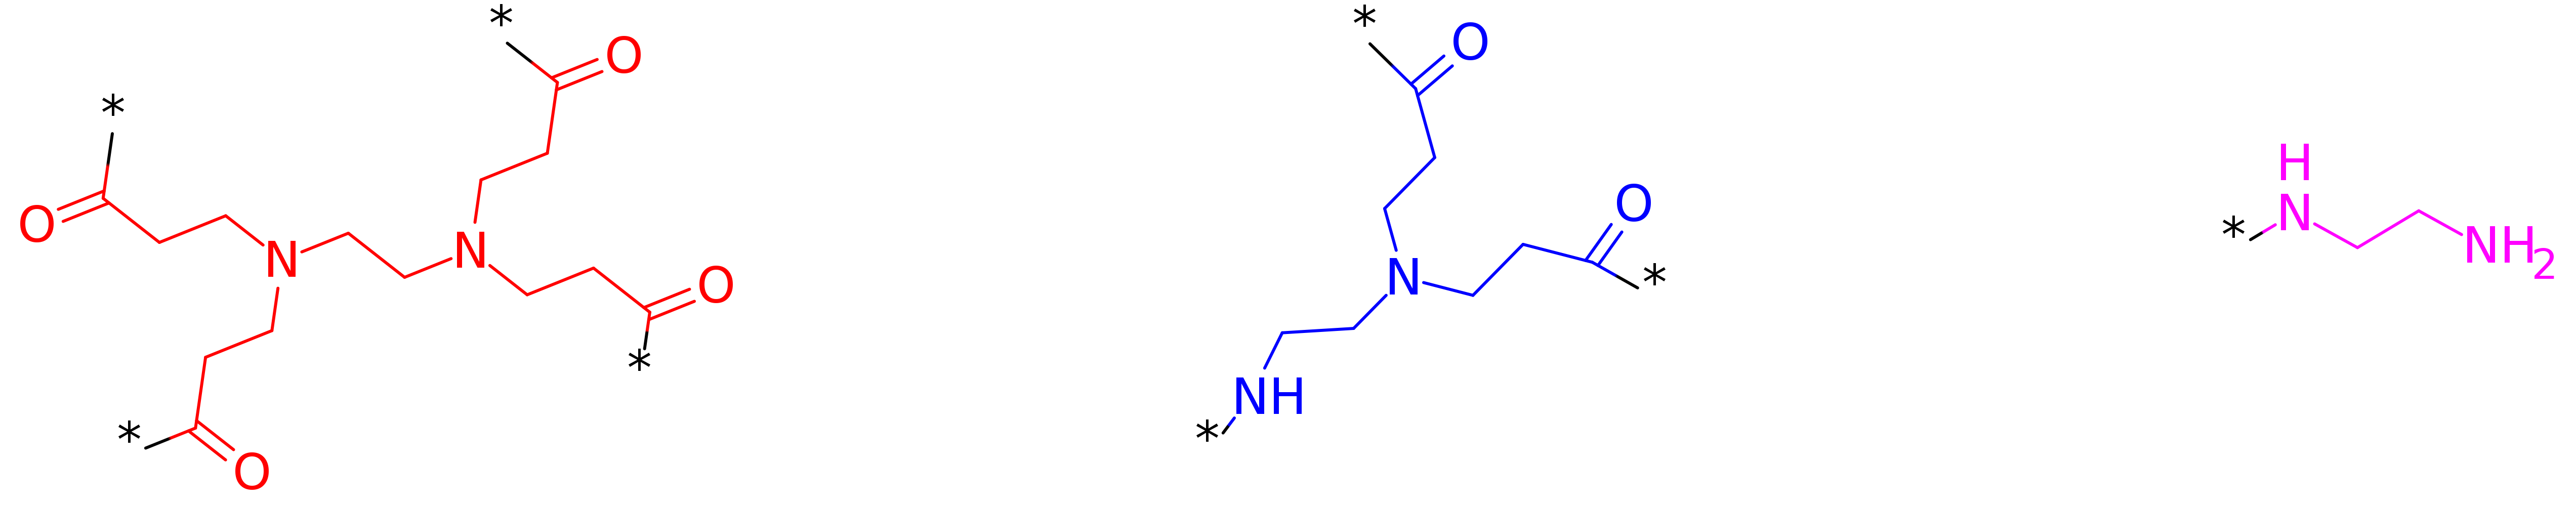
\includegraphics[width=\textwidth]{PAMAM/PAMAMBBs.png}
    \caption{PAMAM dendrimer BBs.
             The core ethylene diamine block is illustrated in red, the intermediary tertiary amine one in blue and the terminal primary amine block is displayed in pink.}
    \label{fig:PAMAMBB}
\end{figure}

The BBs are provided in the demo directory in pypolybuilder root, which structure is illustrated below:
\begin{lstlisting}
<path/to/pypolybuilder>/demo/gromacs_format/dendrimer/PAMAM
\end{lstlisting}
\dirtree{%
.1 PAMAM.
.2 core\_PAMAM.itp.
.2 inter\_PAMAM.itp.
.2 ter\_PAMAM.itp.
.2 list\_param.itp.
.2 run.
.3 PAMAM.sh.
.3 PAMAM.top.
.3 mdp.
}

The file names are self-explanatory, the core\_PAMAM.itp file is the MTF for the core block, the inter\_PAMAM.itp for the intermediary and the ter\_PAMAM.itp, the terminal one.
Once the BBs and the parameters list are successfully built, one can easily run pypolybuilder by using the code line below (also available in file \texttt{how\_to\_run\_this\_example.txt} in demo directory) to obtain a generation 2 PAMAM dendrimer (Figure \ref{fig:PAMAMG2}):

\begin{lstlisting}
python3 ../../../../__main__.py --core=core_PAMAM.itp --inter=inter_PAMAM.itp --ter=ter_PAMAM.itp --params=list_param.itp --ngen=2 --name=PAMAM --output=PAMAM.itp --gro=PAMAM.gro --gromacs --dendrimer
\end{lstlisting}

\begin{figure}
    \centering
    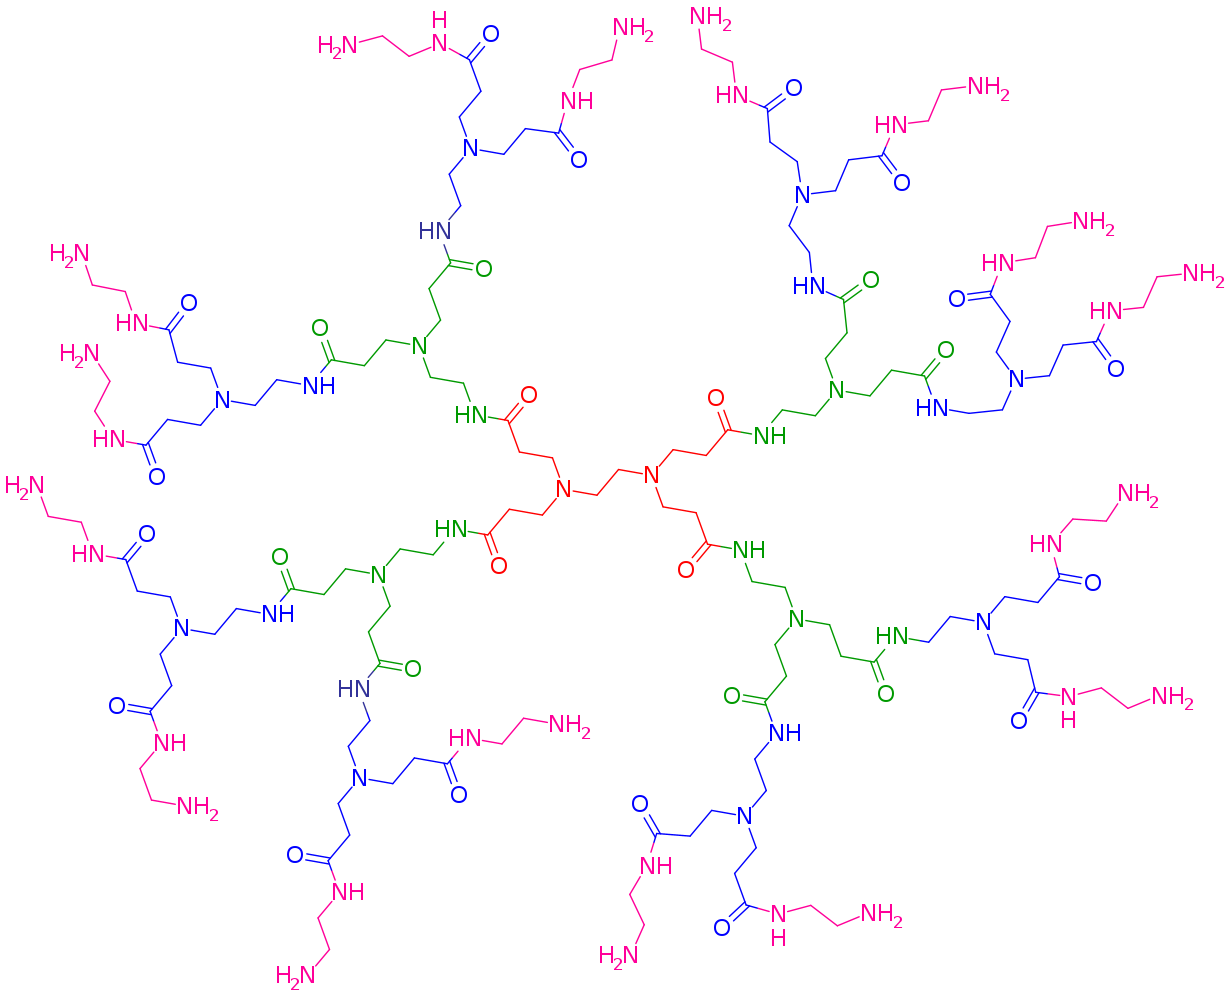
\includegraphics[width=0.5\textwidth]{PAMAM/PAMAMG2.png}
    \caption{PAMAM G2 dendrimer. The color code is the same as the BBs illustrated in Figure \ref{fig:PAMAMBB}.Besides, the first intermediary shell is displayed in green.}
    \label{fig:PAMAMG2}
\end{figure}

The used options in this command line were chosen to select each building block (\texttt{--core}, \texttt{--inter} and \texttt{--ter}), the desired dendrimer generation \texttt{(--ngen}), the name of the topology, for instance the name that will be placed into \texttt{[ moleculetype ]} in the MTF 
(--name), the list of force field parameters for pyPolyBuilder (\texttt{--params}) as well as to name the coordinates and molecular topology output files (\texttt{--gro} and \texttt{--output}, respectively).
Also, the module and the format for the output were selected using, respectively, \texttt{--dendrimer} and \texttt{--gromacs}.

Protonated BBs were also provided and the use of them for creating a protonated PAMAM is left as an exercise.
They have the same file name as the unprotonated BBs but with the suffix ``-protonated''.
Protonated BBs were omitted from the directory tree for simplicity.

After pyPolyBuilder finishes the optimization step, one can use any visualization software to check the output geometry. 
Note that the coordinates are generated considering the molecule in vaccum.
Hence, it may not be the expected solvated conformation (see Figure \ref{fig:PAMAMG2PPB}).
Because of that, the run directory has some scripts to run a short MD simulation in order to equilibrate the molecule in water using gromacs.

\begin{figure}
    \centering
    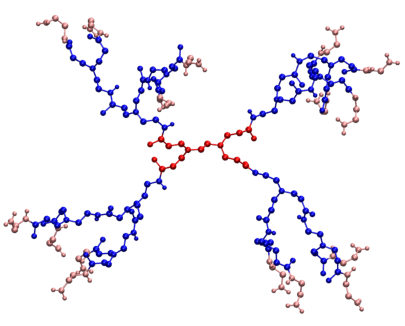
\includegraphics[width=0.5\textwidth]{PAMAM/PAMAM.pdf}
    \caption{Illustration of PAMAM G2 dendrimer generated with pyPolyBuilder.
    The snapshot is displayed in accordance with the previously defined color scheme for the BBs. The core is displayed in red, all intermediary shell monomers are displayed in blue and the terminal blocks are in pink.}
    \label{fig:PAMAMG2PPB}
\end{figure}

In order to test the generated MTF and the initial guess for the geometry, we developed an automated script to simulate this tutorial.
PAMAM.sh is a script to automatically solvate, equilibrate and simulate the molecule built in this tutorial.
Even though the simulated time is not long enough to compute properties consistently, it may be used as basis to future simulations and to evaluate the MTF.
%PAMAM.sh is a script to automatically solvate, minimize energy, equilibrate for 100 ps using nvt and npt ensemble and run 100 ps of molecular dynamic simulation (simulation time is far from the desired for this kind of system. However it may be changed in mdp files. Our main goal is to illustrate the generation of a molecular model using pyPolyBuilder).
PAMAM.top is the topology file for the system and mdp  have all required mdp files.
However, these scripts were developed for a specific architecture and should be adapted by the user.
For instance, the path for gromacs needs to be adapted and the output from pyPolyBuilder (PAMAM.gro and PAMAM.itp) needs to be moved to run directory.

After solvation, an energy minization cycle, 100 ps of nvt equilibration and 100 ps of npt equilibration, the system reaches the conformation illustrated in Figure \ref{fig:PAMAMG2SOL}.

\begin{figure}[ht!]
    \centering
    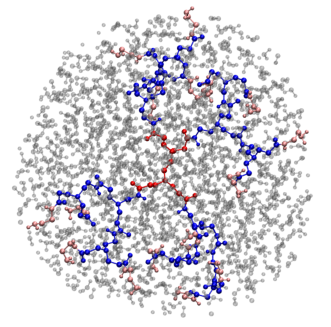
\includegraphics[width=0.5\textwidth]{PAMAM/PAMAMSOL.pdf}
    \caption{Illustration of PAMAM G2 dendrimer. The core is displayed in red, all intermediary shell monomers are displayed in blue and the terminal blocks are in pink.}
    \label{fig:PAMAMG2SOL}
\end{figure}

A powerful feature of the dendrimer module, is that one can easily generate dendrimers of various sizes by only changing one single integer in the input, the \texttt{--ngen}.
Figure \ref{fig:PAMAMGS} illustrate the procedure of varying \texttt{--ngen} from 0 to 5.

\begin{figure}[ht!]
    \centering
    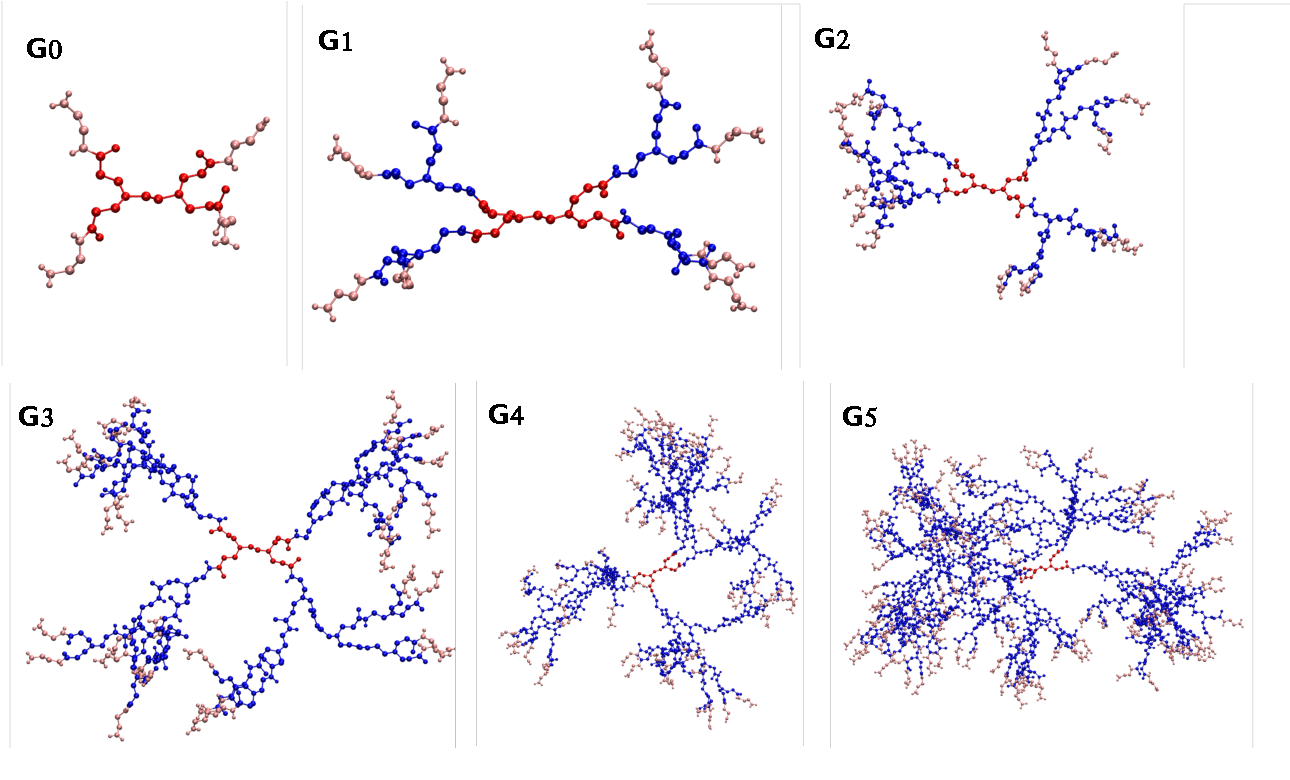
\includegraphics[width=\textwidth]{PAMAM/PAMAMGs.pdf}
    \caption{PAMAM dendrimer from generations 0 to 5 built by using pyPolyBuilder and varying the \texttt{--ngen} option only between each run.
    Color scheme is in accordance with Figure \ref{fig:PAMAMBB}, that is, the core is displayed in red, all shells of intermediary monomers are in blue and terminal blocks are in pink.}
    \label{fig:PAMAMGS}
\end{figure}
\clearpage

\subsubsection{PPI}

The BBs for the poly(propyleneimine) (PPI) dendrimer are shown in Figure \ref{fig:PPIBB}.
The core is a diamino butane, intermediary monomer is defined as a tertiary amine in addition to a secondary amine, which is the anchoring point for the core or previous intermediary shell bonding and the terminal is simply a primary amine.
It is important to note that PPI dendrimers are commonly defined differently.
For instance, this tutorial may be adapted to generate a common used PPI dendrimer by removing the secondary amine from the intermediary monomer and modifying the \texttt{[ branches ]} field in \texttt{inter\_PPI.itp}.

\begin{figure}
    \centering
    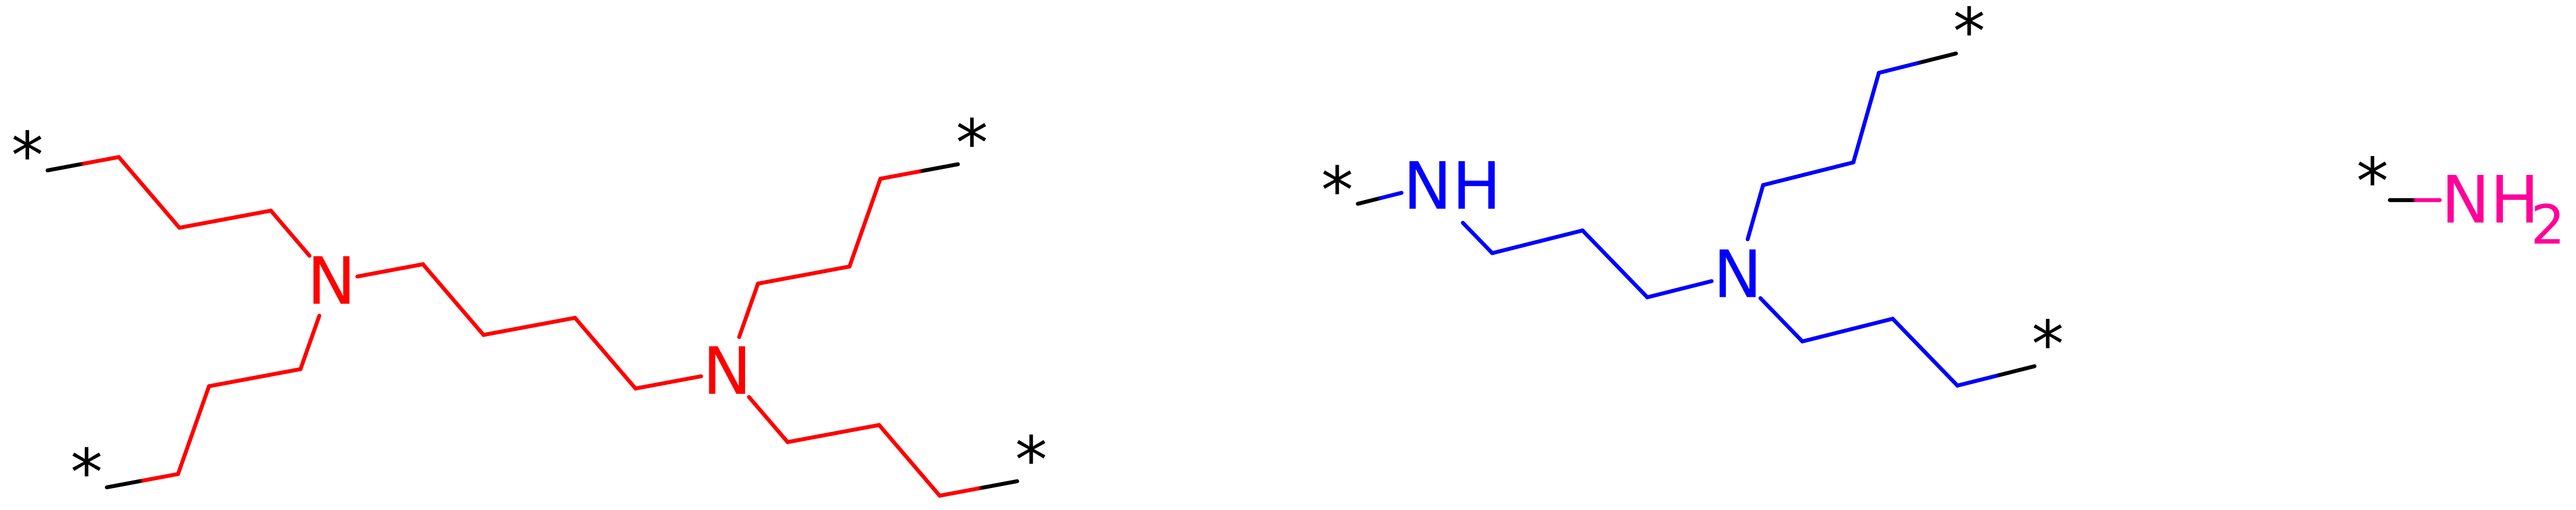
\includegraphics[width=\textwidth]{PPI/PPIBBs.png}
    \caption{PPI dendrimer BBs.
             The core diamine butane block is illustrated in red, the intermediary tertiary amine in blue and the terminal primary amine block is displayed in pink.}
    \label{fig:PPIBB}
\end{figure}

All PPI BBs, in addition to their protonated versions, are provided in the demo directory in pypolybuilder root, whose structure is illustrated beelow:
\begin{lstlisting}
<path/to/pypolybuilder>/demo/gromacs_format/dendrimer/PPI
\end{lstlisting}
\dirtree{%
.1 PPI.
.2 core\_PPI.itp.
.2 inter\_PPI.itp.
.2 ter\_PPI.itp.
.2 list\_param.itp.
.2 run.
.3 PPI.sh.
.3 PPI.top.
.3 mdp.
}

The core\_PPI.itp, inter\_PPI.itp, and ter\_PPI.itp files are the MTF for the core, the intermediary, and the terminal blocks, respectively.
Once the BBs and the parameters list are successfully built, one can easily run pyPolyBuilder by using the code line (also available in \texttt{how\_to\_run\_this\_example.txt} in demo directory) to obtain a generation 1 PPI dendrimer (Figure \ref{fig:PPIG1}):

\begin{lstlisting}
python3 ../../../../__main__.py \
--core=core_PPI.itp \
--inter=inter_PPI.itp \
--ter=ter_PPI.itp \
--params=list_param.itp \
--ngen=1 \
--name=PPI \
--output=PPI.itp \
--gro=PPI.gro \
--dendrimer
\end{lstlisting}

Each option in this command line was chosen to select each building block (\texttt{--core}, \texttt{--inter} and \texttt{--ter}),  the dendrimer generation \texttt{(--ngen}), the topology name, for instance the name that will be placed into \texttt{[ moleculetype ]} in the MTF 
(--name), to parse the list of force field parameters for pyPolyBuilder (\texttt{--params}), and to name the coordinates file and MTF output (\texttt{--gro} and \texttt{--output}, respectively).

\begin{figure}
    \centering
    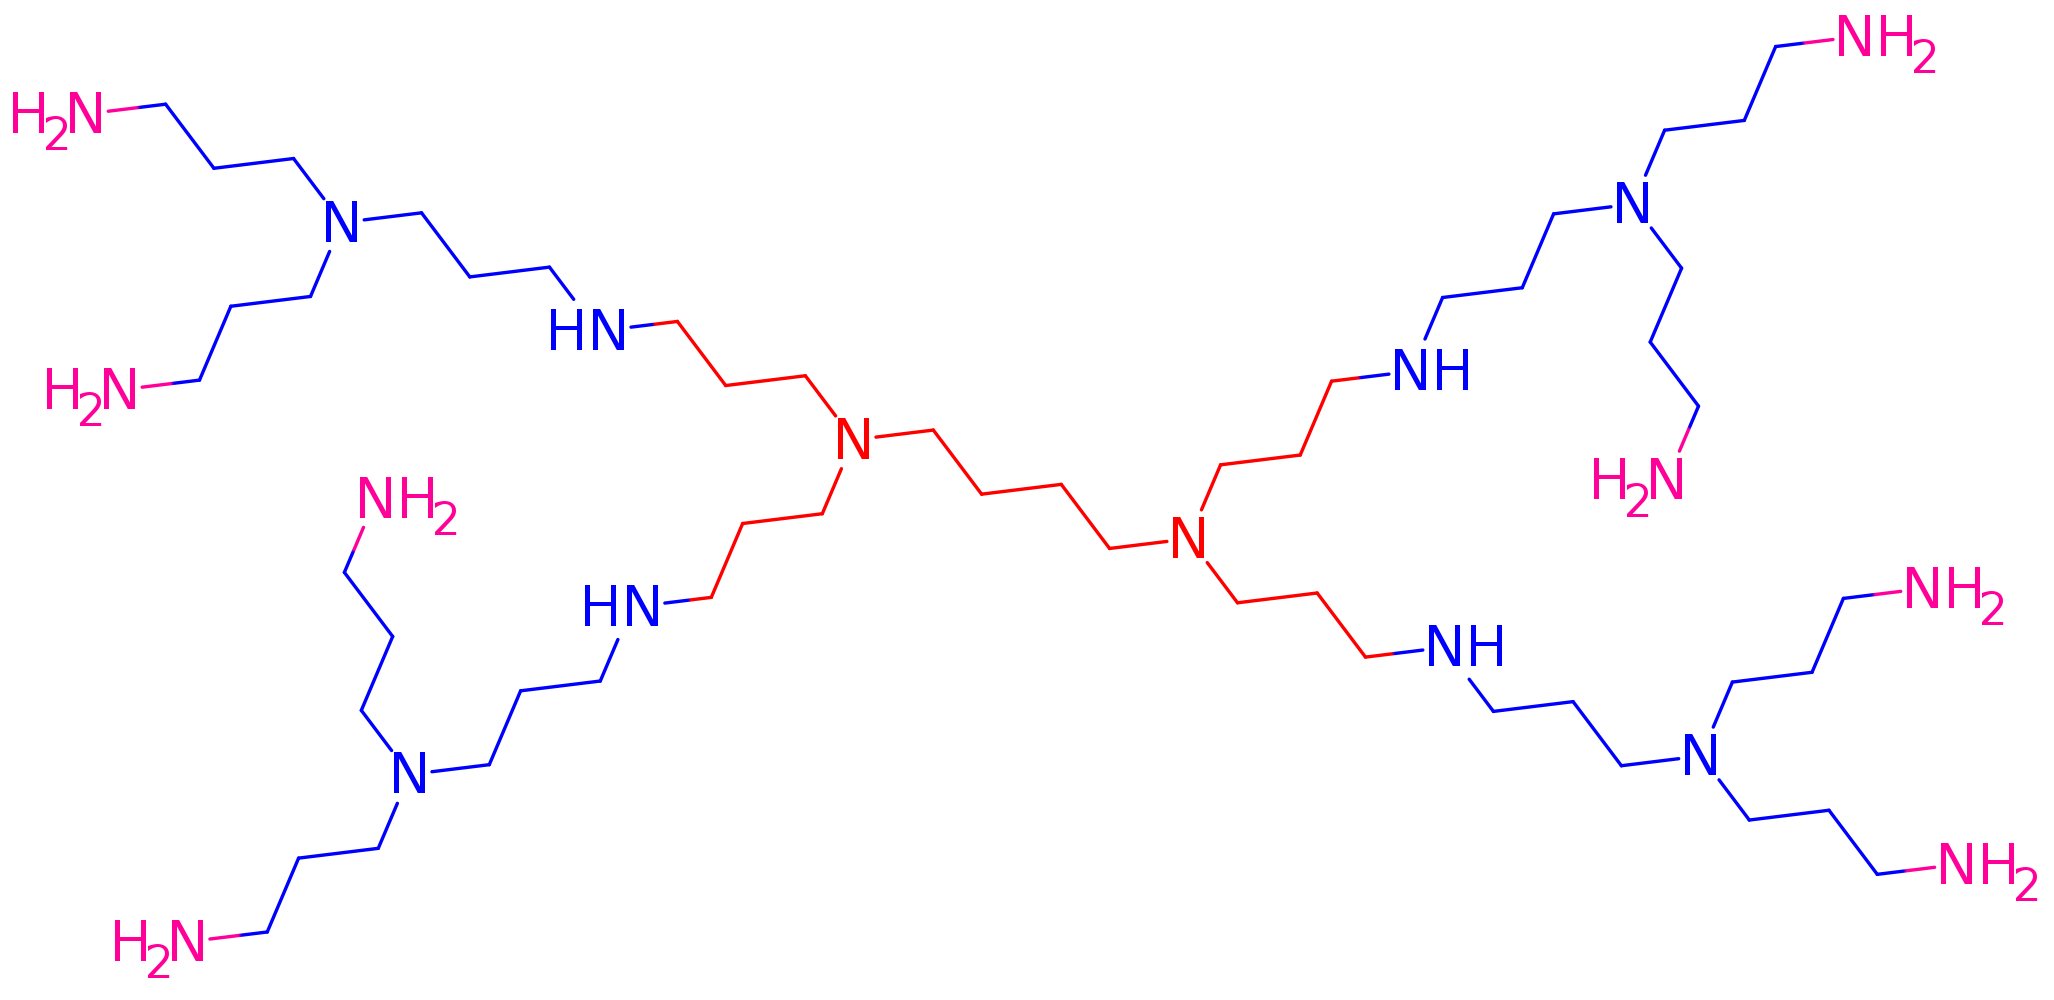
\includegraphics[width=0.5\textwidth]{PPI/PPIG1.png}
    \caption{PPI G1 dendrimer.
             The color code is adopted from Figure \ref{fig:PPIBB}.}
    \label{fig:PPIG1}
\end{figure}

It is worth noticing that protonated BBs were also provided.
The interested user is welcome to use them.
They have the same file name than the unprotonated BBs but with the suffix ``-protonated''.
Protonated BBs were omitted from the directory tree for simplicity.

After pyPolyBuilder finished the optimization step, any visualization software can be used to check the output geometry. 
Since the coordinates are generated considering the molecule in vaccum, its conformation may not be the expected solvated one (see Figure \ref{fig:PPIG1PPB}).
For that reason, the run directory has some scripts to run a short MD simulation in order to equilibrate the molecule in water using gromacs.
However, these scripts were developed for a specific architecture and need to be adapted by each user.

\begin{figure}
    \centering
    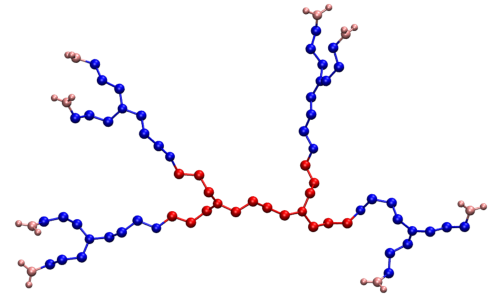
\includegraphics[width=0.5\textwidth]{PPI/PPI.pdf}
    \caption{PPI G1 dendrimer built by pyPolyBuilder.
             The color code is the same as in Figure \ref{fig:PPIBB}.}
    \label{fig:PPIG1PPB}
\end{figure}

PPI.sh is a script to automatically solvate, minimize energy, equilibrate for 100 ps using nvt and npt ensemble, and run 100 ps of molecular dynamic simulation.
The simulation time is actually too small for simulating dendrimers. With this tutorial, we only intend to illustrate how pyPolyBuilder can be used in the creation of a molecular model.
PPI.top is the topology file for the system and mdp directory have all required mdp files.
However, these scripts were developed for a specific architecture and need to be adapted by each user.
For instance, the path for gromacs needs to be adapted and the output from pyPolyBuilder (PPI.gro and PPI.itp) needs to be moved to run directory.

After carrying out the solvation, energy minimization, and 100 ps of both nvt and npt equilibrations, PPI dendrimer is in a more reasonable conformation (Figure \ref{fig:PPIG1SOL}).

\begin{figure}
    \centering
    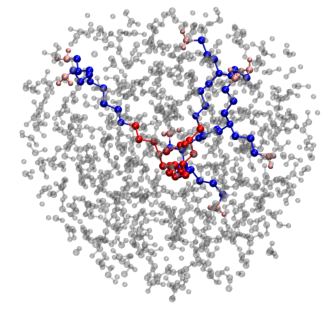
\includegraphics[width=0.5\textwidth]{PPI/PPISOL.pdf}
    \caption{PPI G1 dendrimer in water solution.
             The color code is the same as in Figure \ref{fig:PPIBB}.
             Water molecules are represented as translucent gray molecules.}
    \label{fig:PPIG1SOL}
\end{figure}
\clearpage

\subsubsection{SPL7013}

Dendrimers of the SPL family are a challenging test case for pyPolyBuilder.
Among the examples considered in this tutorial, this is the most complex case for the dendrimer module.
Its structure for a generation 1 dendrimer is illustrated in Figure \ref{fig:SPL7013G1}.

\begin{figure}
    \centering
    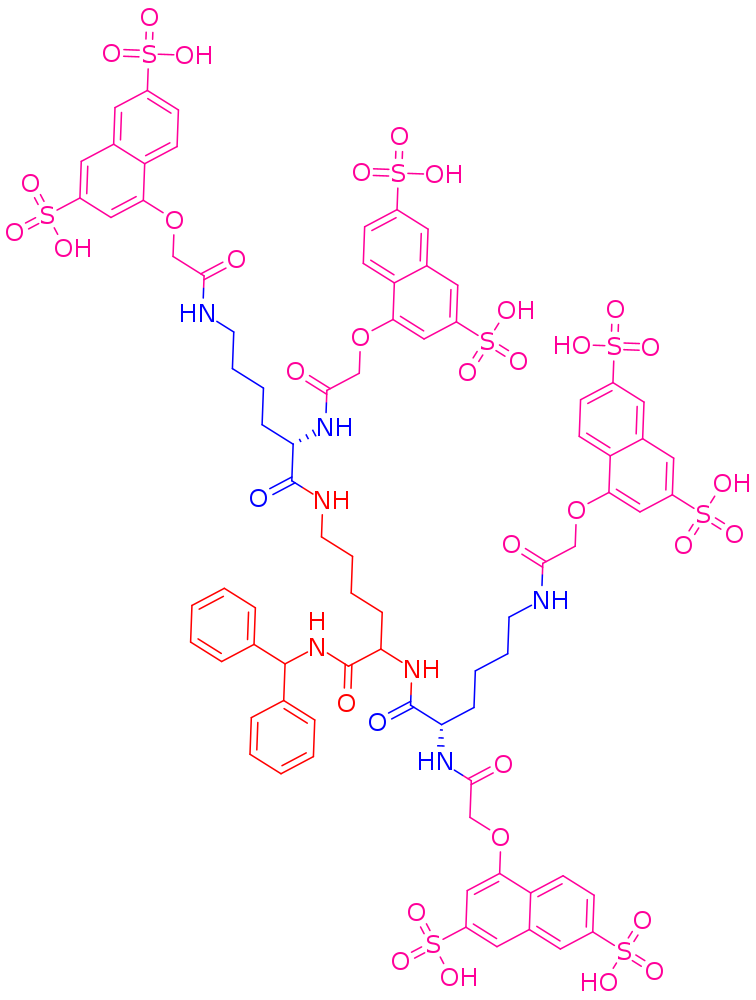
\includegraphics[width=0.5\textwidth]{SPL7013/SPL7013G1.png}
    \caption{SPL G1 dendrimer.
            The benzhydrylamine core is illustrated in red, the intermediaries lysine is in blue and the terminals naphthalene disulfonate acid is in pink.
             }
    \label{fig:SPL7013G1}
\end{figure}

The division for the SPL BBs was made as the colors suggest in Figure \ref{fig:SPL7013G1}.
The benzhydrylamine bonded to a lysine is chosen to be the core, a lysine molecule alone is the intermediary block and the napthtalene disulfonate is the terminal block.
The BBs themselves are illustrated in Figure \ref{fig:SPL7013BB}.

\begin{figure}
    \centering
    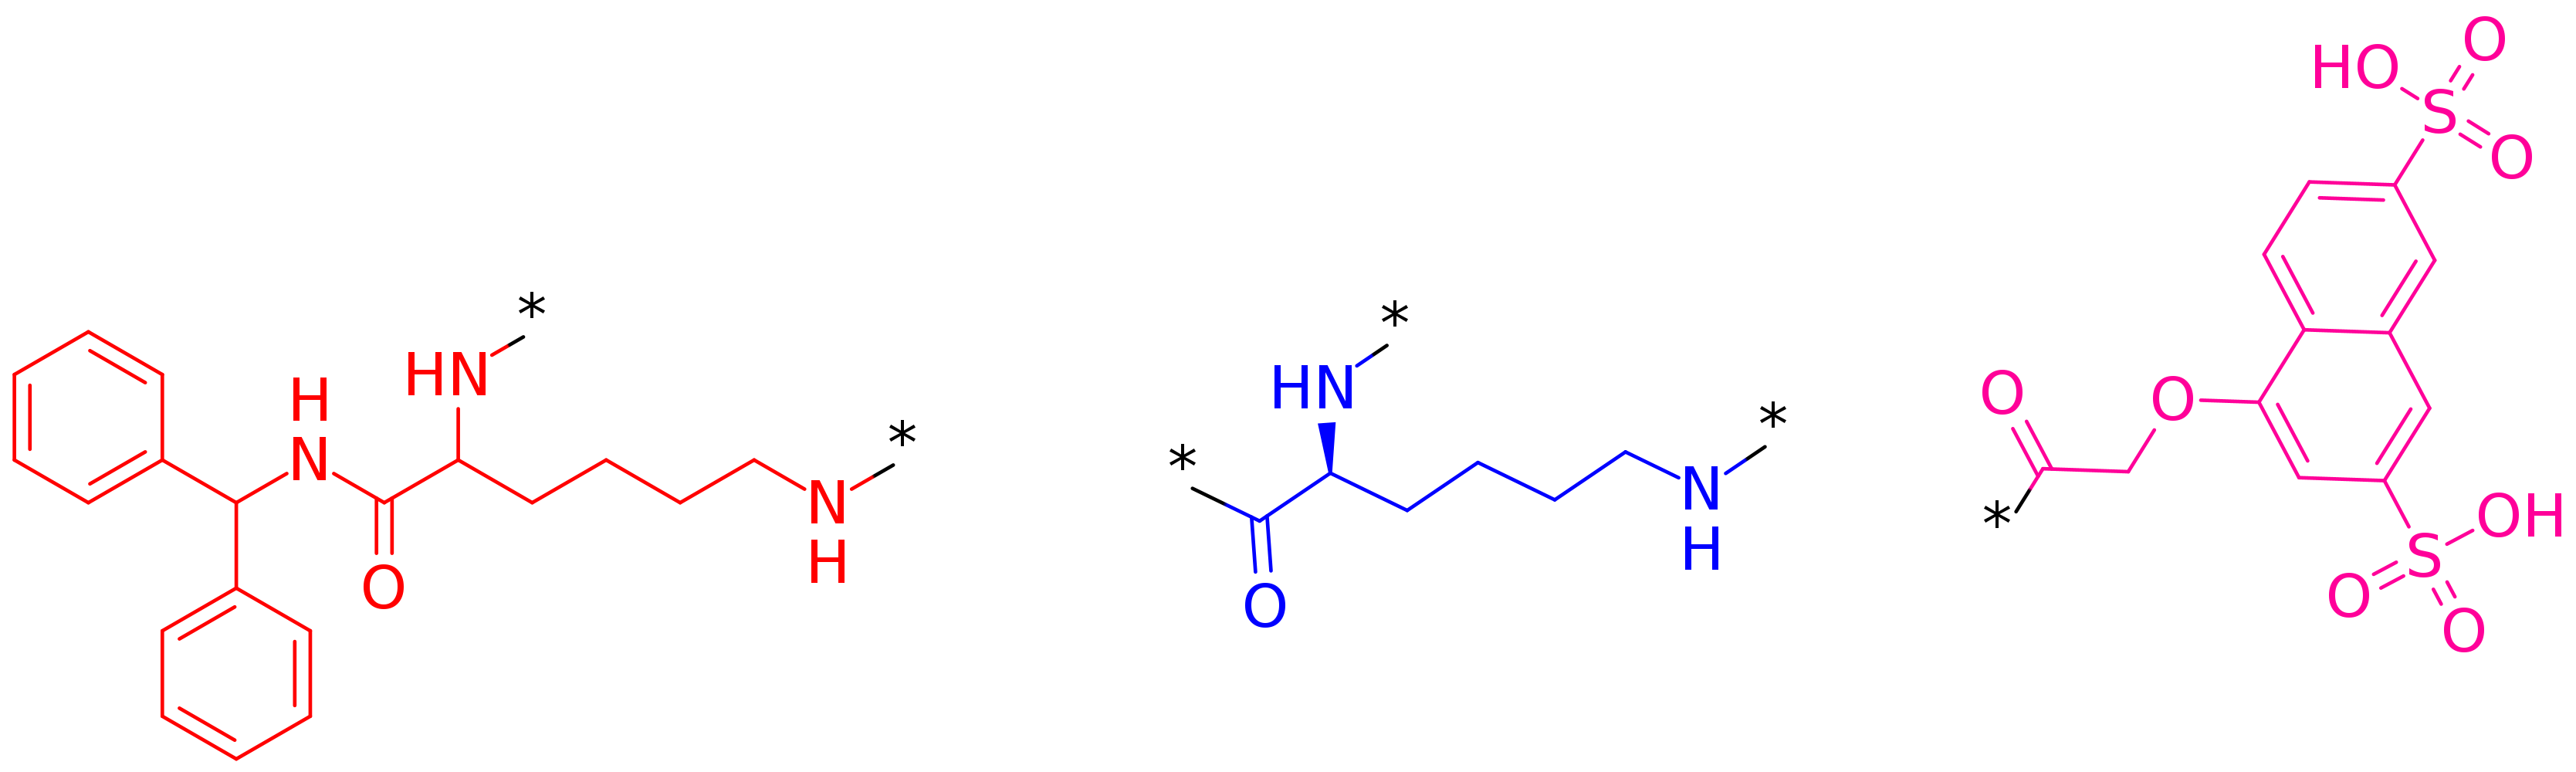
\includegraphics[width=\textwidth]{SPL7013/SPL7013BBs.png}
    \caption{SPL7013 dendrimer BBs.
             The colors were chosen to match the ones illustrated in Figure \ref{fig:SPL7013G1}.}
    \label{fig:SPL7013BB}
\end{figure}

MTFs for those BBs are available in the tutorial directory in pyPolyBuilder root, which structure is illustrated below:
\begin{lstlisting}
<path/to/pypolybuilder>/demo/gromacs_format/dendrimer/SPL7013
\end{lstlisting}
\dirtree{%
.1 SPL7013.
.2 core\_BHA.itp.
.2 inter\_LYS.itp.
.2 ter\_NDSA.itp.
.2 list\_param.itp.
.2 run.
.3 SPL7013.sh.
.3 SPL7013.top.
.3 mdp.
}

The MTFs are named according to its block and molecule name.
The core\_BHA.itp is the benzhydrylamine core BB, inter\_LYS.itp the lysine intermediary block and the ter\_NDSA.itp is the naphtalene disulfonate acid terminal block.

The command line below can be used to build a generation 1 SPL dendrimer (Figure \ref{fig:SPL7013G1}):

\begin{lstlisting}
python3 ../../../../__main__.py --core=core_BDA.itp --inter=inter_LYS.itp --ter=ter_NDSA.itp --params=list_param.itp --ngen=1 --name=SPL --output=SPL.itp --gro=SPL.gro --nsteps=5000 --nskipLJ=100 --gromacs --stepLength=0.0001 --forcefield=../../../../gromos2016h66.ff --dendrimer
\end{lstlisting}

Some of the used option were already used in previous tutorials and explained in Section \ref{sec:CommandLine}.
\texttt{--core}, \texttt{--inter} and \texttt{--ter} are used to select the dendrimer BBs and \texttt{--ngen} to select its generation number.
\texttt{--name}, \texttt{--output} and \texttt{--gro} are used to name the topology, the MTF itself and the geometry coordinates file, respectively.
\texttt{--gromacs} is used to define the format of the output files, in this case, in the gromacs format.
Even though \texttt{--gromacs} is the default, \texttt{--gromos} is also available.
\texttt{--nsteps} set how many steps will be made in geometry optimization step.
PyPolyBuilder stops the iteration if the energy converges or if the \texttt{nstep} is reached.
Before doing a local minimization to carry the geometry to a local minimum, pyPolyBuilder carry out a genetic algorithm (GA) optimization only for the torsional dihedrals in order to set a initial quasi-optimum geometry that will be optimized in the local minimization step.
Due to the stochastic nature of GA, in very complex geometries it is possible that some atoms are very close at the end of the GA optimization.
To avoid these bad interactions, \texttt{--nSkipLJ} set how many steps of the geometry optimization will be carried out without evaluating Lennard-Jones (LJ) interactions.
Turning LJ interactions off for the first few steps allows the structure to relax only using bonded potentials avoiding bad contacts.
\texttt{--stepLength} set the size of the minimization step.
Also for complex systems, it is possible that the output of GA is far from optimum.
So \texttt{--stepLength} can be used to allow a slow minimization in order to avoid overlaps.
pyPolyBuilder has default values for bonded and non-bonded parameters.
Because of that, the generated structure may not actually be at the minimum of the desired force field.
Using the \texttt{--forceField} flag, one can pass to pyPolyBuilder the location of a force field (FF) in gromacs format to be used in the geometry optimization. 
It may be possible in some cases that the built-in FF is not good enough.

SPL is, for instance, a real challenge due to its very complex structure.
In this tutorial, 2016H66 FF was used to optimize its geometry, the built-in FF lead to an unphysical geometry in which some of the bonds were too long and others were too short (it can be tested by removing the \texttt{--forcefield} flag from the previous command-line).
Besides, the obtained structure may be equally problematic if the \texttt{--nsteps} keyword is not used.

This is a really specific and singular dendrimer.
The fact that the pyPolyBuilder is able to build this structure proofs its versatility and robustness.

After pyPolyBuilder finish the optimization step, one can use any visualization software (such as vmd or pymol) to check the output geometry. 
Note that the coordinates are generated considering a dendrimer without any partial charge in vaccum.
Hence, the obtained conformation is probably not fully realistic.
However, if one wants to test the topology of this purely academic case, the run directory has some scripts to run a short molecular dynamics in order to equilibrate the molecule in water using gromacs.
These scripts were developed for a specific architecture and should be adapted by the user.

\begin{figure}
    \centering
    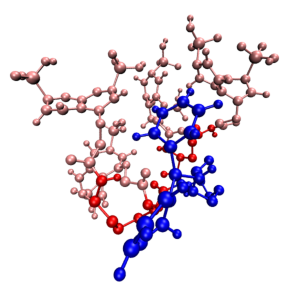
\includegraphics[width=0.5\textwidth]{SPL7013/SPL1.pdf}
    \caption{SPL G1 dendrimer built by pyPolyBuilder.
             The colors were chosen to match Figure \ref{fig:SPL7013G1}.}
    \label{fig:SPL7013PPB}
\end{figure}

Using the available scripts in the run directory to run a small equilibration after solvation and energy minimization in gromacs package, one can see the structure of SPL G1 dendrimer in Figure \ref{fig:SPL7013SOL}.

\begin{figure}
    \centering
    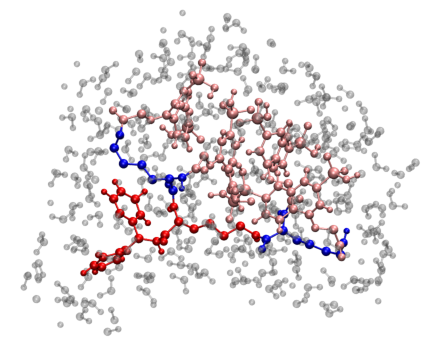
\includegraphics[width=0.5\textwidth]{SPL7013/SPLSOL.pdf}
    \caption{SPL G1 dendrimer equilibrated in water.
             The colors were chosen to match Figure \ref{fig:SPL7013G1}.
             Water molecules are illustrated as the translucent gray molecules.}
    \label{fig:SPL7013SOL}
\end{figure}


\clearpage

\subsubsection{PAMAM/PPI-Janus}
\label{PAMAM/PPI-Janus}

A Janus dendrimer is a amphiphilic dendrimer in which the hydrophobic part is concentrated in a side while the hydrophilic part is concentrated in the opposite side.
We illustrated this kind of molecule by concentrating the PAMAM BBs in one region and the PPI BBs at the opposite region of the resulting dendrimer, as depicted in Figure \ref{fig:JanusG1}.
This way, the resulting dendrimer is not amphiphilic due to the similar nature of the PAMAM and PPI chemistry, yet it is a Janus-like dendrimer since it is split into two dendrimeric parts.
At the present approach, we used only the dendrimer module for building a method inspired by the divergent synthesis method for creating Janus-like dendrimers.
We illustrate this method by using PAMAM and PPI dendrimers BBs.

\begin{figure}
    \centering
    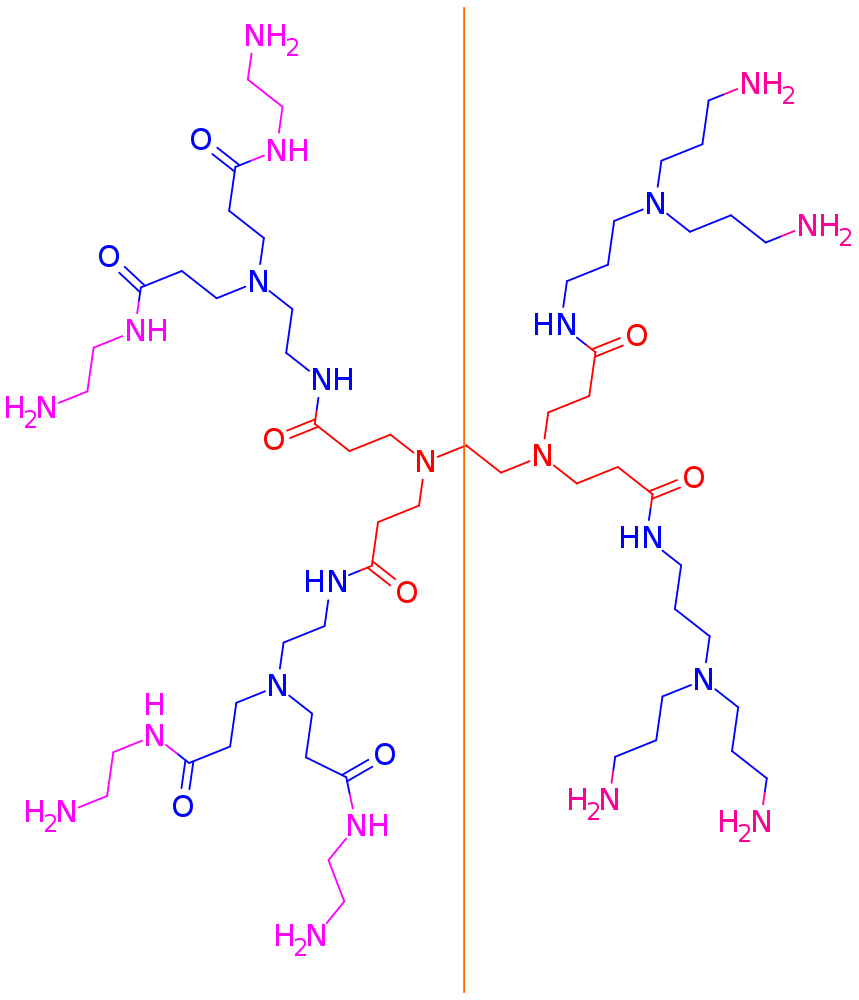
\includegraphics[width=0.5\textwidth]{PAMAM_PPI-Janus/JANUSG1.png}
    \caption{PAMAM/PPI Janus G1 dendrimer.}
    \label{fig:JanusG1}
\end{figure}

The dendrimer module was designed for building homogeneous perfect dendrimers.
Hence, it is not straightforward to build a dendrimer using BBs of different types.
The BBs that are going to be used in this tutorial are exactly the same ones used in previous tutorials (see Figure \ref{fig:JanusBBs}).
These files are provided in the demo directory in pypolybuilder root, whose structure is illustrated below:
\begin{lstlisting}
<path/to/pypolybuilder>/demo/gromacs_format/dendrimer/PAMAM_PPI
\end{lstlisting}
\dirtree{%
.1 PAMAM\_PPI.
.2 core\_PAMAM.itp.
.2 inter\_PAMAM.itp.
.2 ter\_PAMAM.itp.
.2 inter\_PPI.itp.
.2 ter\_PPI.itp.
.2 list\_param.itp.
.2 run.
.3 PAMAM\_PPI.sh.
.3 PAMAM\_PPI.top.
.3 mdp.
}

\begin{figure}
    \centering
    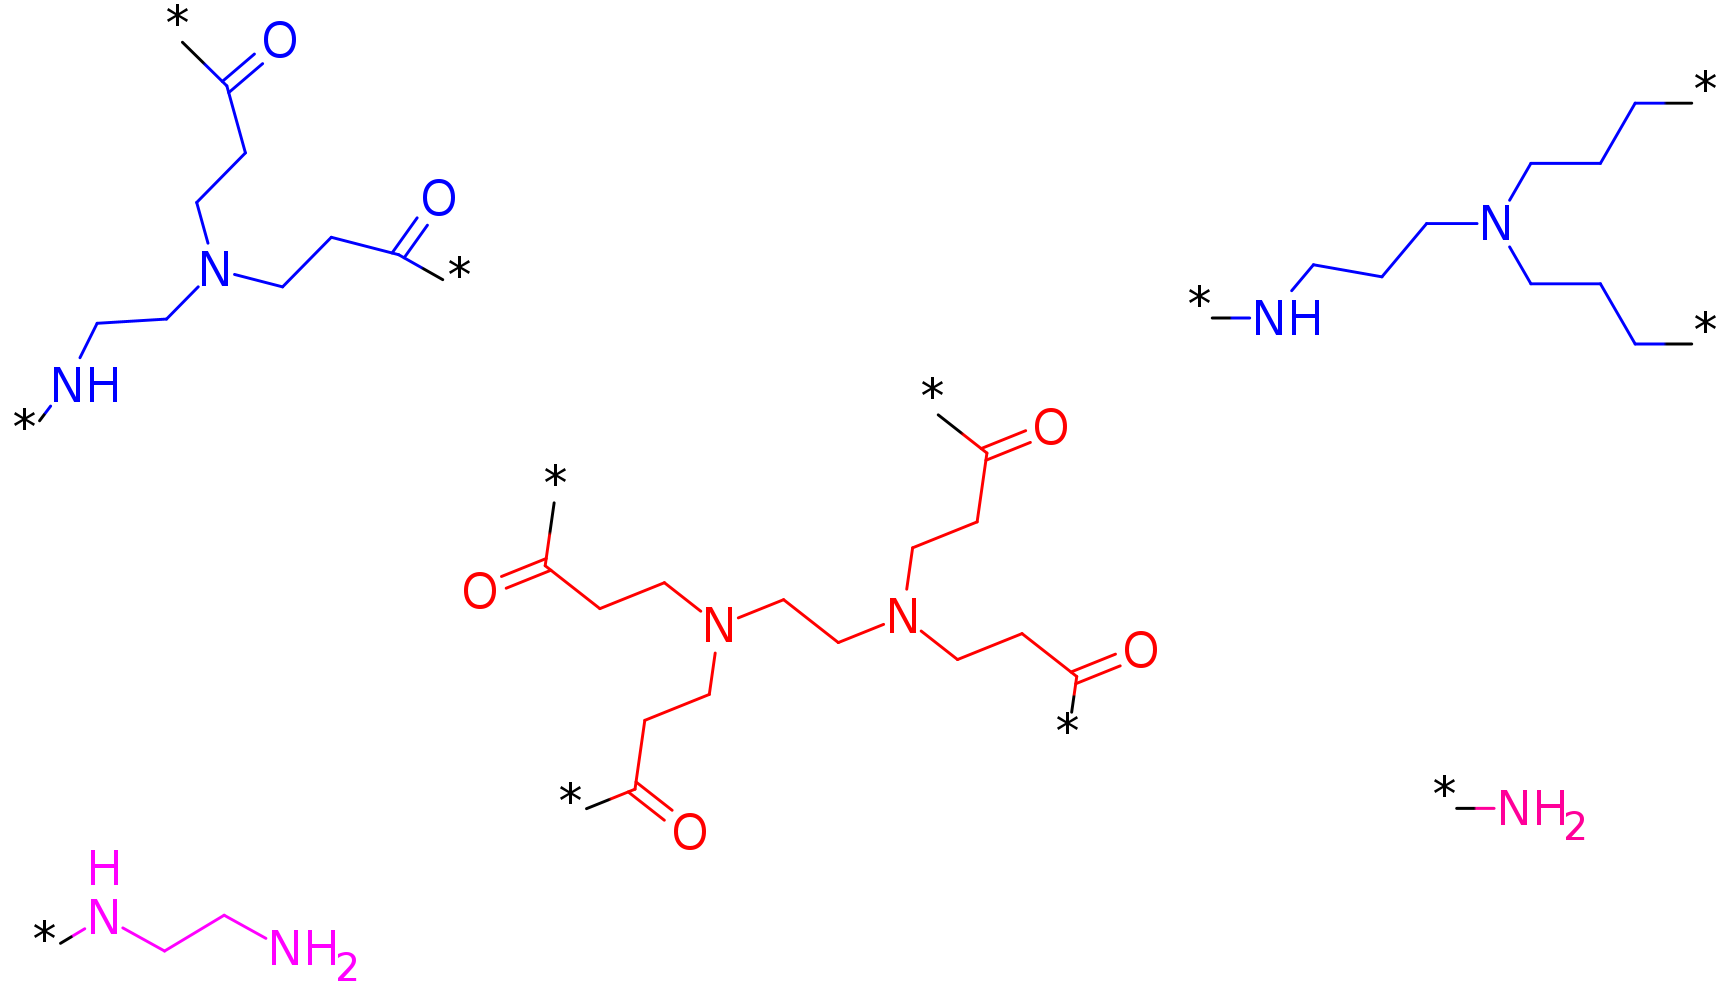
\includegraphics[width=\textwidth]{PAMAM_PPI-Janus/JANUSBBs.png}
    \caption{PAMAM/PPI Janus dendrimer BBs. The PAMAM core block is illustrated in red, intermediary and core blocks are placed on the left in blue and red, respectively. On the right, the BBs for PPI intermediary and core, also in blue and red, respectively.}
    \label{fig:JanusBBs}
\end{figure}

In order to build a Janus dendrimer, we need to make it in two steps.
The whole process is automated in \texttt{how\_to\_run\_this\_example.txt}.
Therefore, this file may be executed with bash in order to get the final geometry.
Nevertheless, the process is described in the following.
First, we need to grow one half of the dendrimer without growing the opposite half.
Afterwards, we use the pyPolyBuilder to grow the second half.
The pyPolyBuilder connects the branches using the dendrimer module according to the \texttt{[ branches ]} field.
The atom indexes in the ``acceptor'' column will receive a new bond from the atom in the ``donor'' column in the incoming new intermediary block.
Therefore, we can edit this field in order to select which branches will be created in each step.
The \texttt{core\_PAMAM.itp} file in this tutorial has its \texttt{[ branches ]} field edited as shown below:

\begin{lstlisting}
[ branches ]
;  donor   acceptor
;   0     10
;   0     13
    0     16
    0     19
\end{lstlisting}

Lines that begin with ``;'' are comments and will not be interpreted by pyPolyBuilder.
With this \texttt{[ branches ]}, the intermediary blocks will only be connected at atoms 16 and 19, respectively.
First, the PAMAM branches are included by using the command line code:

\begin{lstlisting}
python3 ../../../../__main__.py \
--core=core_PAMAM.itp \
--inter=inter_PAMAM.itp \
--ter=ter_PAMAM.itp \
--params=list_param.itp \
--ngen=1 \
--name=PAMH \
--output=PAMAMhalf.itp \
--nogeom \
--dendrimer
\end{lstlisting}

In this command line, \texttt{--core}, \texttt{--inter} and \texttt{--ter} were used for selecting the building blocks, \texttt{--params} for parsing force fields parameter files, \texttt{--ngen} to select the generation of the PAMAM that will be grown, \texttt{--name} for naming the topology, and \texttt{--output} for naming the generated MTF.
Notice that the option \texttt{--gro} was not used here since the geometry will not be optimized and an initial guess for the geometry will not be produced.
Accordingly, we use the \texttt{--nogeom} flag.
As this is just an intermediary step in the process of creating the molecule, only the MTF is needed.
See the Section \ref{sec:CommandLine}.
After the build is done, a new \texttt{PAMAMhalf.itp} MTF with the PAMAM half of the Janus dendrimer (Figure \ref{fig:JanusPAMAMhalf}) will be produced.

\begin{figure}
    \centering
    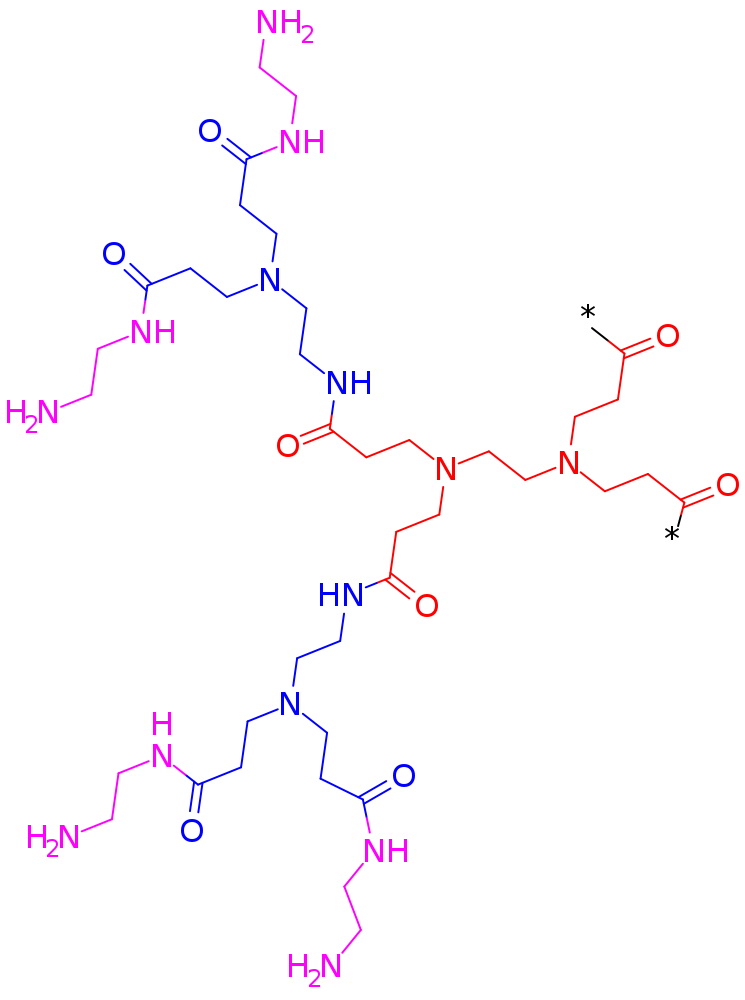
\includegraphics[width=0.4\textwidth]{PAMAM_PPI-Janus/JANUSPAMAMhalf.png}
    \caption{The dendrimer with only the PAMAM BBs attached to the core BB.}
    \label{fig:JanusPAMAMhalf}
\end{figure}

The PAMAM core has 4 branch points, at the atoms 10, 13, 16 and 19.
We have already used the branch points 16 and 19 for growing the part in which we used the PAMAM BBS.
However, the atoms 10 and 13 are available for growing the second half of the dendrimer using the PPI BBs.
We need to edit the \texttt{PAMAMhalf.itp} file
to include the desired \texttt{[ branches ]} shown below in the final of the file:

\begin{lstlisting}
[ branches ]
;  donor   acceptor
    0     10
    0     13
;   0     16
;   0     19
\end{lstlisting}

After editing the \texttt{PAMAMhalf.itp} file, the second part of the dendrimer may be grown by running the following command line:

\begin{lstlisting}
python3 ../../../../__main__.py \
--core=PAMAMhalf.itp \
--inter=inter_PPI.itp \
--ter=ter_PPI.itp \
--params=list_param.itp \
--ngen=1 \
--name=PAMPPI \
--output=PAMAM_PPI.itp \
--gro=PAMAM_PPI.gro \
--dendrimer
\end{lstlisting}

Here, as the geometry is wanted, the \texttt{--nogeom} flag was not used.
Instead, \texttt{--gro} option was used to name the gro file that will be generated.

After pyPolyBuilder has finished the optimization step, one can use any visualization software to check the output geometry. 
Note that the coordinates are generated considering the molecule in vaccum.
Hence, it may not be the expected conformation in solvent (Figure \ref{fig:JanusPPB}).
Because of that, the run directory has some scripts to run a short MD simulation in order to equilibrate the molecule in water using gromacs.
However, these scripts were developed for a specific architecture and needs to be adapted by the user.

\begin{figure}
    \centering
    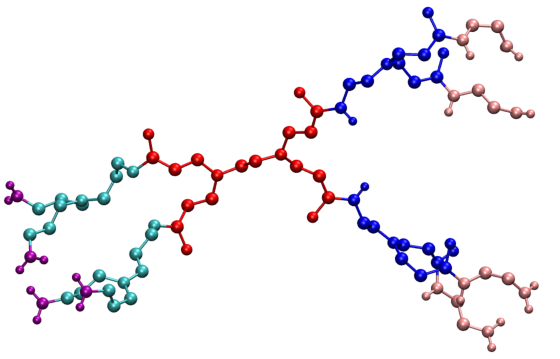
\includegraphics[width=0.5\textwidth]{PAMAM_PPI-Janus/PAMAM_PPI.pdf}
    \caption{The Janus-like dendrimer generated by pyPolyBuilder using PAMAM and PPI BBs. The PAMAM core is displayed in red, PAMAM and PPI intermediaries are displayed, respectively, in blue and cyan, and the terminal PAMAM and PPI blocks are in pink and purple, respectively.
    For instance, in this snapshot, the PAMAM half is at the right side of the structure, and PPI half at the left side.}
    \label{fig:JanusPPB}
\end{figure}

Using the topology generated by pyPolyBuilder, the Janus-like dendrimer was solvated, its energy was minimized, and equilibrations in nvt and npt ensembles were carried out for 100 ps each (Figure \ref{fig:JanusSOL}).

\begin{figure}
    \centering
    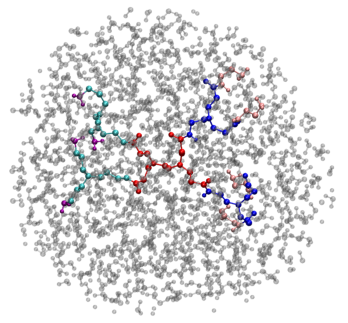
\includegraphics[width=0.5\textwidth]{PAMAM_PPI-Janus/PAMAM_PPISOL.pdf}
    \caption{The created Janus-like structure after equilibration in water solvent.
    Similarly to the Figure \ref{fig:JanusPPB}, PAMAM monomers are at the right side of the molecule while PPI monomers are at the left side, at this snapshot.
    The color scheme was chosen to be the same as in Figure \ref{fig:JanusPPB}.}
    \label{fig:JanusSOL}
\end{figure}

\clearpage

\subsection{Network module}
Differently from the dendrimer module, there is no pre-assumed polymer topology.
Hence, the user needs to completely define how every BB is connected.
In order to make all information about the molecule connectivity available in one single file, the network module does not use the \texttt{[ branches ]} field.
Besides, all the connections should be passed in the connectivity file through the \texttt{--in} option.
Its content was already discussed in Section \ref{sec:GENinputFiles}.
Also, when using this module, all the building blocks should be passed using the \texttt{--bbs} option (differently from dendrimer module that uses the options \texttt{--core}, \texttt{--inter} and \texttt{--ter}).

Here we provide some simple tutorials aiming to give the user some prototype files and to pass the philosophy of using the network module of pyPolyBuilder.

\subsubsection{PEG}

Poly ethyleneglycol (PEG) polymer is made by multiple ethyleneglycol monomers.
Each monomer for building PEG in this tutorial was chosen to be the oxygen atom plus its two neighbor atoms in accordance to the GROMOS united atoms FF (Figure \ref{fig:PEGBBs}).

\begin{figure}
    \centering
    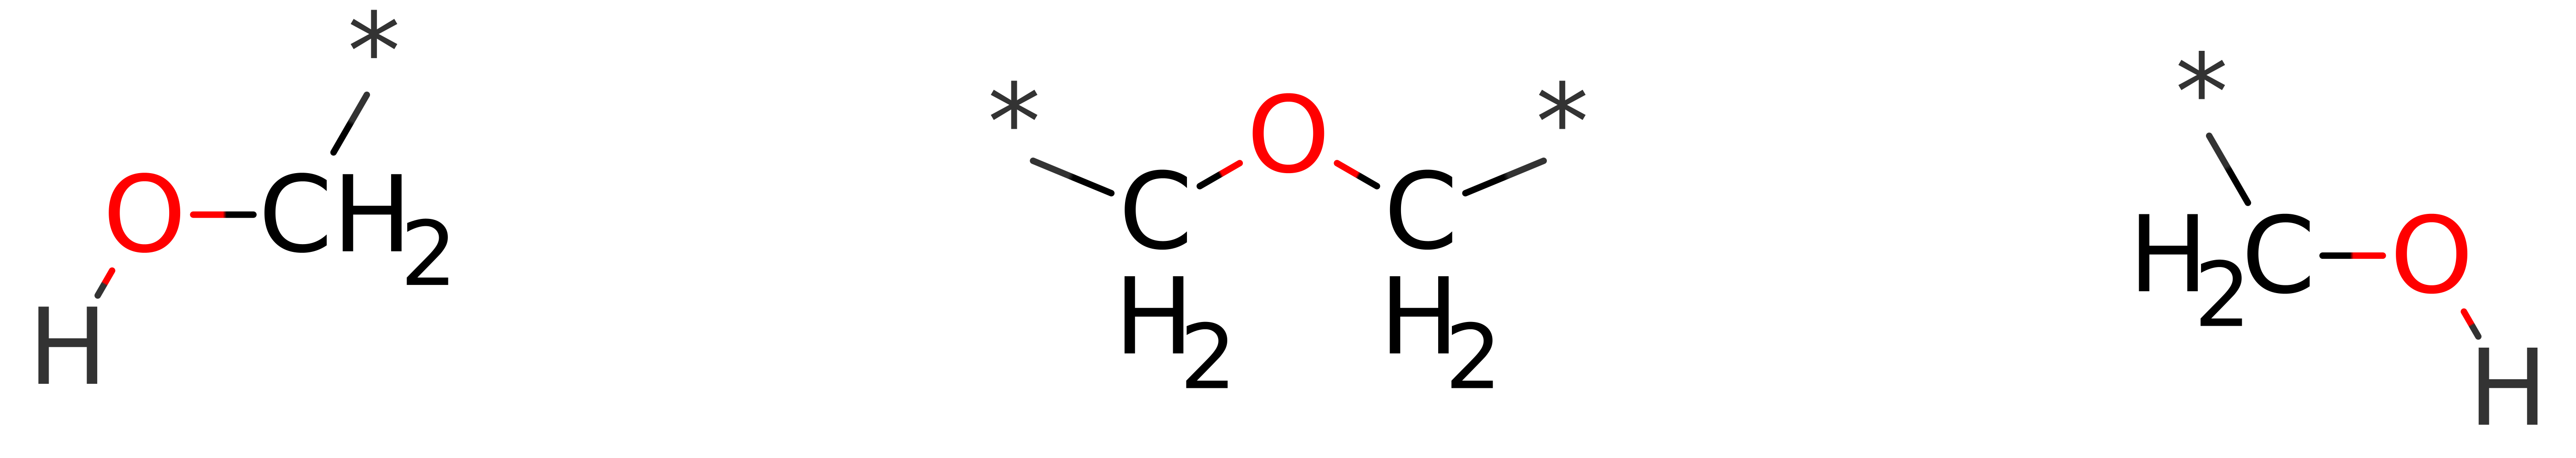
\includegraphics[width=\textwidth]{PEG/PEGBBs.png}
    \caption{PEG BBs. The left and the right monomers are the initial and final monomers, respectively.
            The middle one is the repeating monomer unit.}
    \label{fig:PEGBBs}
\end{figure}

The monomers are pretty simple to be build due to the small number of atoms that need to be defined.
The building blocks as defined in Figure \ref{fig:PEGBBs} are available in the tutorial directory as bb\_PNIP-start.itp, bb\_PNIP.itp and bb\_PNIP-end.itp.

All needed files are provided in the demo directory in pyPolyBuilder root.
\begin{lstlisting}
<path/to/pypolybuilder>/demo/gromacs_format/polymer/PolyEthylene_glycol
\end{lstlisting}
\dirtree{%
.1 PEG.
.2 polyeyhylene-start.itp.
.2 polyeyhylene.itp.
.2 polyeyhylene-end.itp.
.2 list\_param.itp.
.2 connect.in.
.2 connect-4.in.
.2 run.
.3 PEG.sh.
.3 PEG.top.
.3 mdp.
}

The command for building a PEG polymer with 5 monomers is automated in a bash file within tutorial directory called \texttt{how\_to\_run\_this\_example.txt}.
% \begin{figure}
%     \center
%     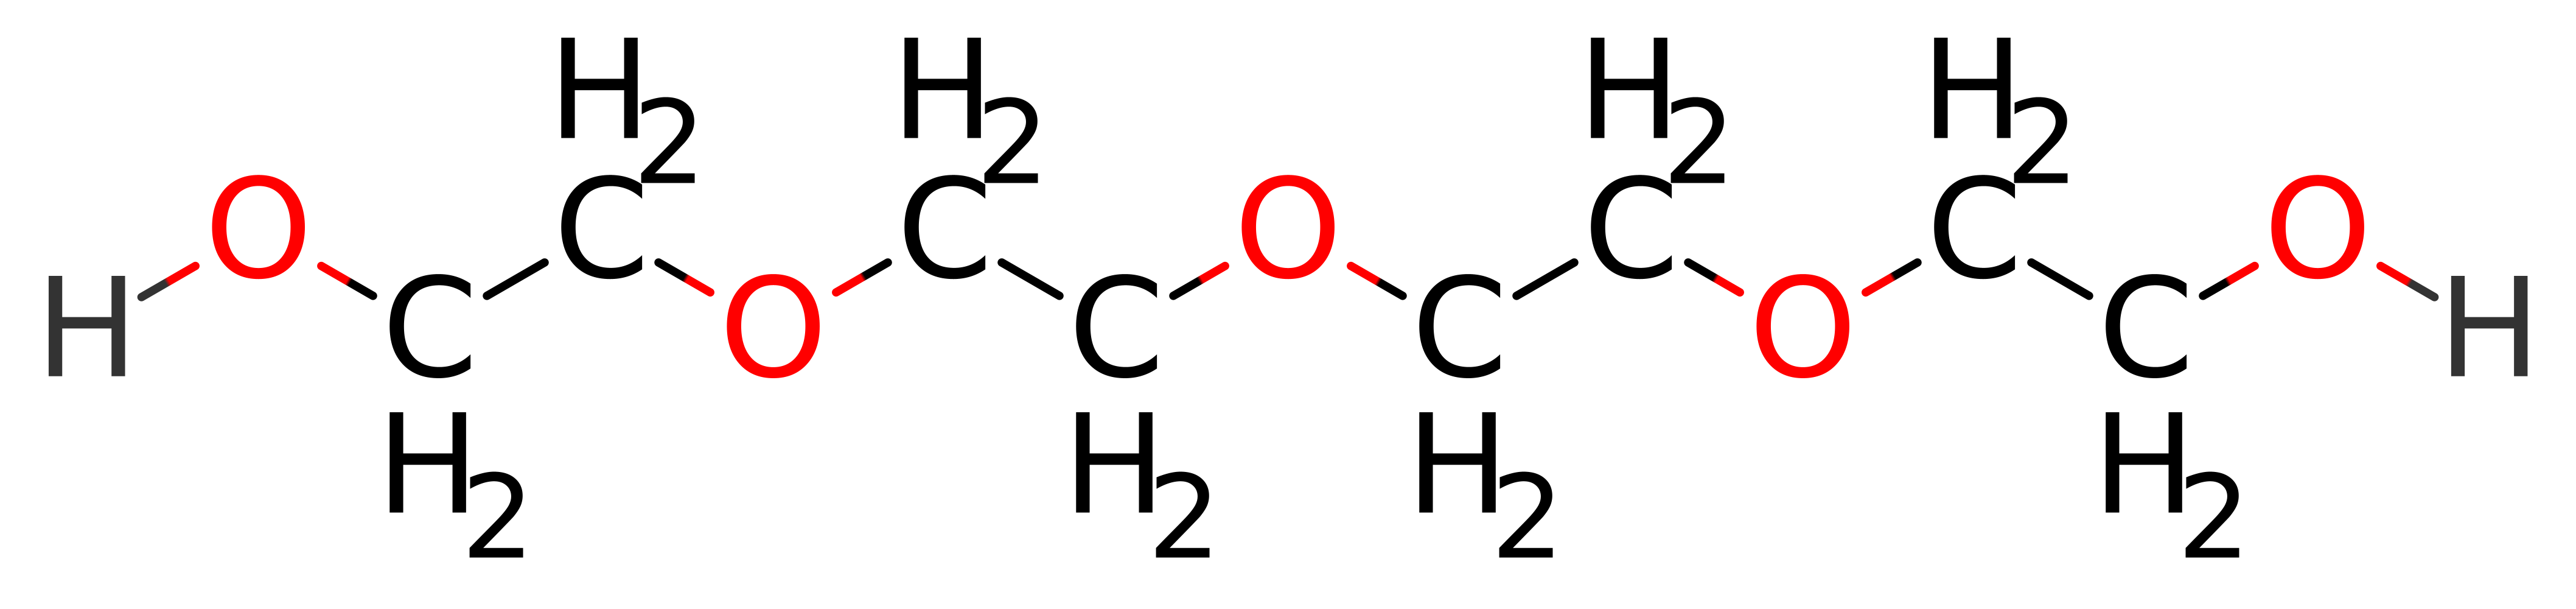
\includegraphics[width=0.5\textwidth]{PEG/PEG.png}
%     \caption{The PEG polymer in the way it is built in this tutorial.}
%     \label{fig:PEG}
% \end{figure}

In order to have a PEG polymer with 5 monomers, with the files provided in the tutorial directory one can use the following command line:

\begin{lstlisting}
python3 ../../../../__main__.py \
   --bbs=etyleneglycol-start.itp,etyleneglycol.itp,etyleneglycol-end.itp \
   --in=connect.in \
   --params=list_param.itp \
   --name=PEG \
   --output=PEG5x.itp \
   --gro=PEG5x.gro \
   --network
\end{lstlisting}

Here, \texttt{--bb} option receives the three used BBs: the beginning of the polymer, than the repetition monomer and a final BB.
The connectivity file (named "connect.in") is input through \texttt{--in} option.
FF parameters are defined in \texttt{list\_param.itp} used in \texttt{--params}.
Also, the output is named according to \texttt{--name}, \texttt{--output} and \texttt{--gro}.
At this tutorial, the \texttt{--network} flag needs to be used so the network module will be called.

After pyPolyBuilder has finished the optimization step, one can check the molecule geometry in vacuum (Figure \ref{fig:PEGPPB}). 
This initial geometry and the MTFs can be tested by running a MD simulation using the created files.
A script automating a workflow to solvate the polymer and  run a small MD simulation is included in the tutorial directory.

\begin{figure}
    \center
    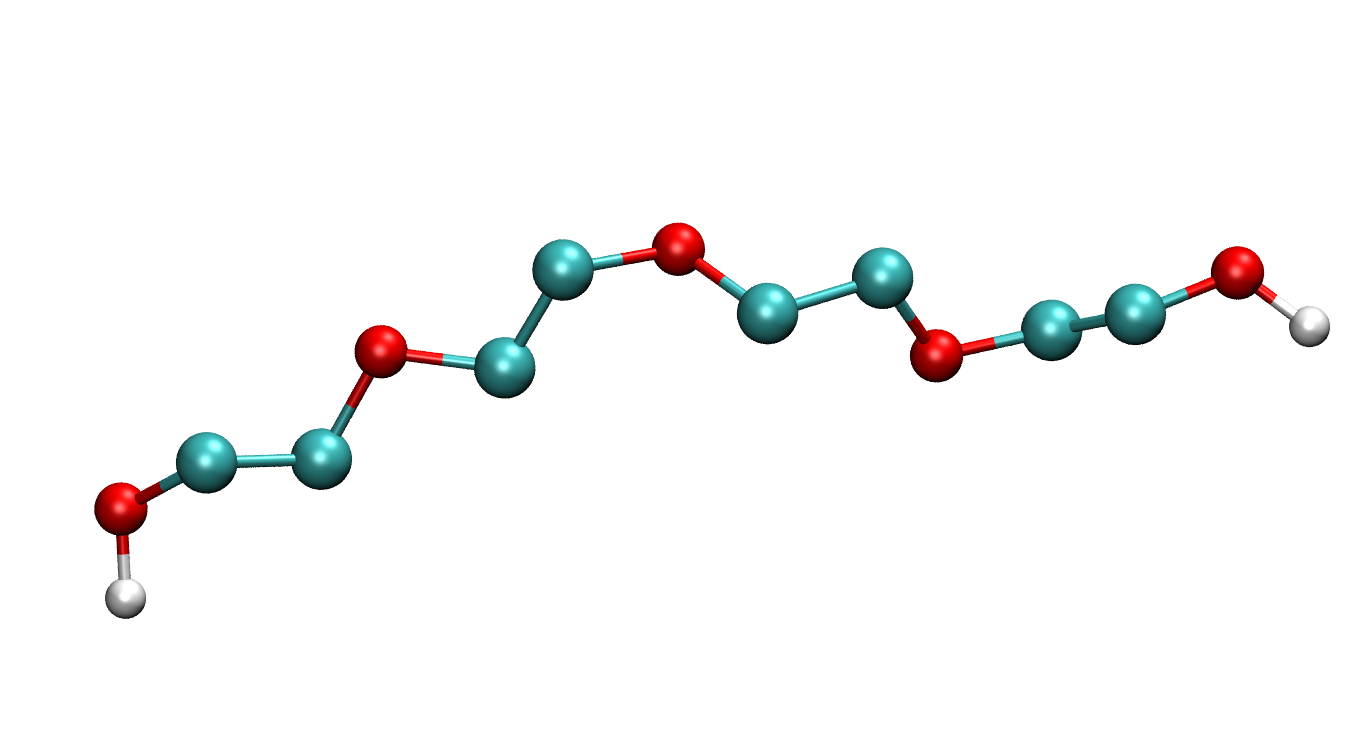
\includegraphics[width=0.5\textwidth]{PEG/PEGPPB.png}
    \caption{The PEG polymer in the way it is built in this tutorial.}
    \label{fig:PEGPPB}
\end{figure}

PEG.sh has the workflow automated but the \texttt{PEG5x.gro} and \texttt{PEG5x.itp} need to be moved to the run directory within tutorial directory and the script needs to be edited in order to use a actual gromacs path on your computer.

Once equilibrated, PEG polymer conformation can be seen as in Figure \ref{fig:PEGSOL}

\begin{figure}
    \center
    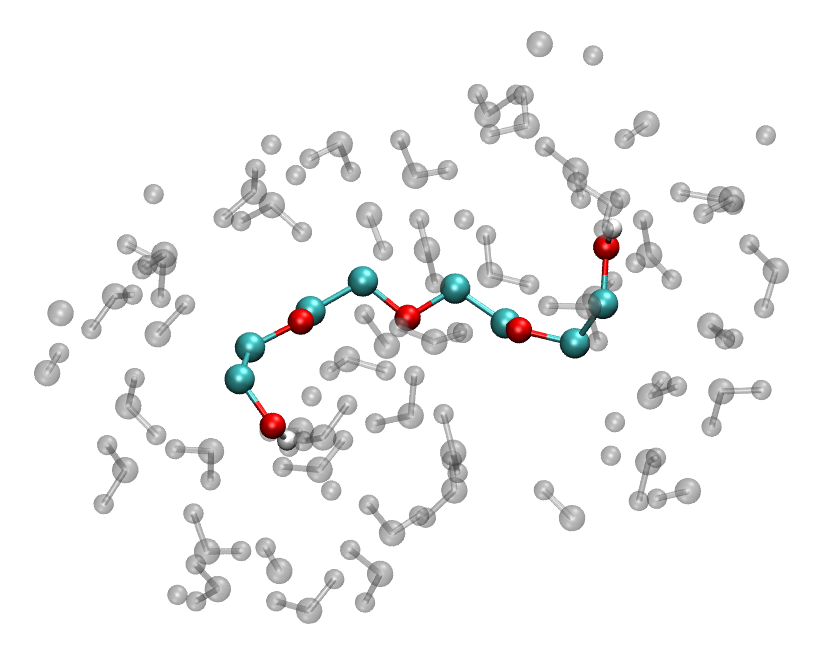
\includegraphics[width=0.5\textwidth]{PEG/PEGSOL.png}
    \caption{The PEG polymer in the way it is built in this tutorial. Water molecules are displayed as translucent silver molecules.}
    \label{fig:PEGSOL}
\end{figure}
\clearpage

\subsubsection{PNIPAM}

The PNIPAM polymer, as it is going to be built in this tutorial, has its monomers as illustrated in Figure \ref{fig:PNIPAMPOL}.
Since the connectivity of the first and last monomers are slightly different (shown in Figure \ref{fig:PNIPAMBBs} by the asterisks), three very similar BBs were created for building PNIPAM.
%All three BBs are illustrated in Figure \ref{fig:PNIPAMBBs}.
The BBs are provided in the demo directory in pypolybuilder root, which structure is illustrated in Figure \ref{fig:PNIPAMBBs}:
Note that the only difference between each BB is the number of carbon atoms in the backbone.

\begin{figure}
    \center
    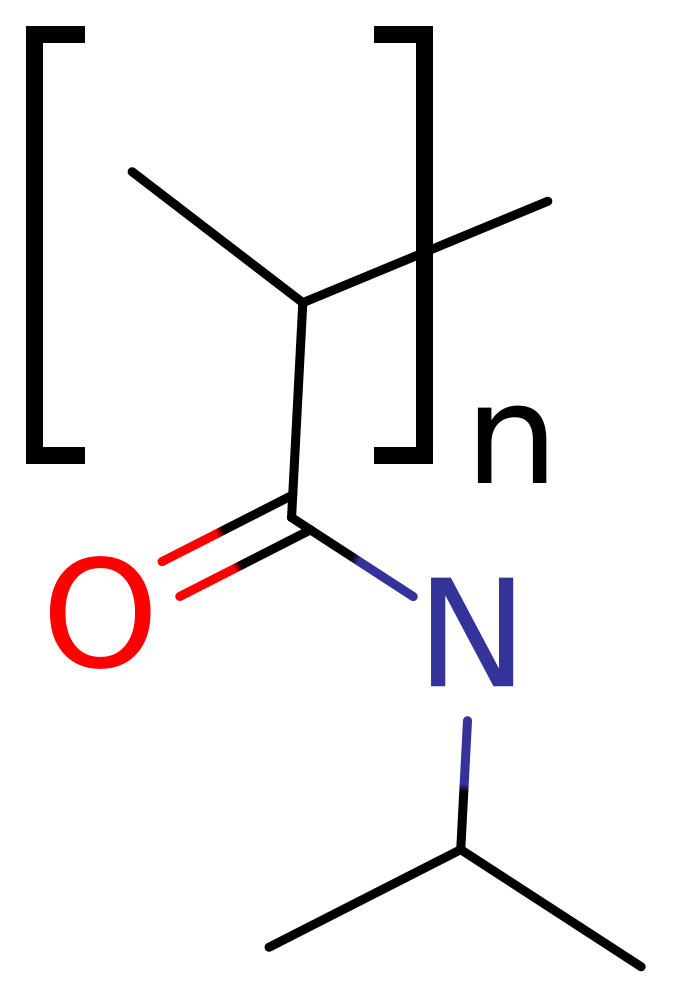
\includegraphics[width=0.3\textwidth]{PNIPAM/PNIPAMPOL.png}
    \caption{The PNIPAM polymer in the way it is built in this tutorial.}
    \label{fig:PNIPAMPOL}
\end{figure}

\begin{figure}
    \centering
    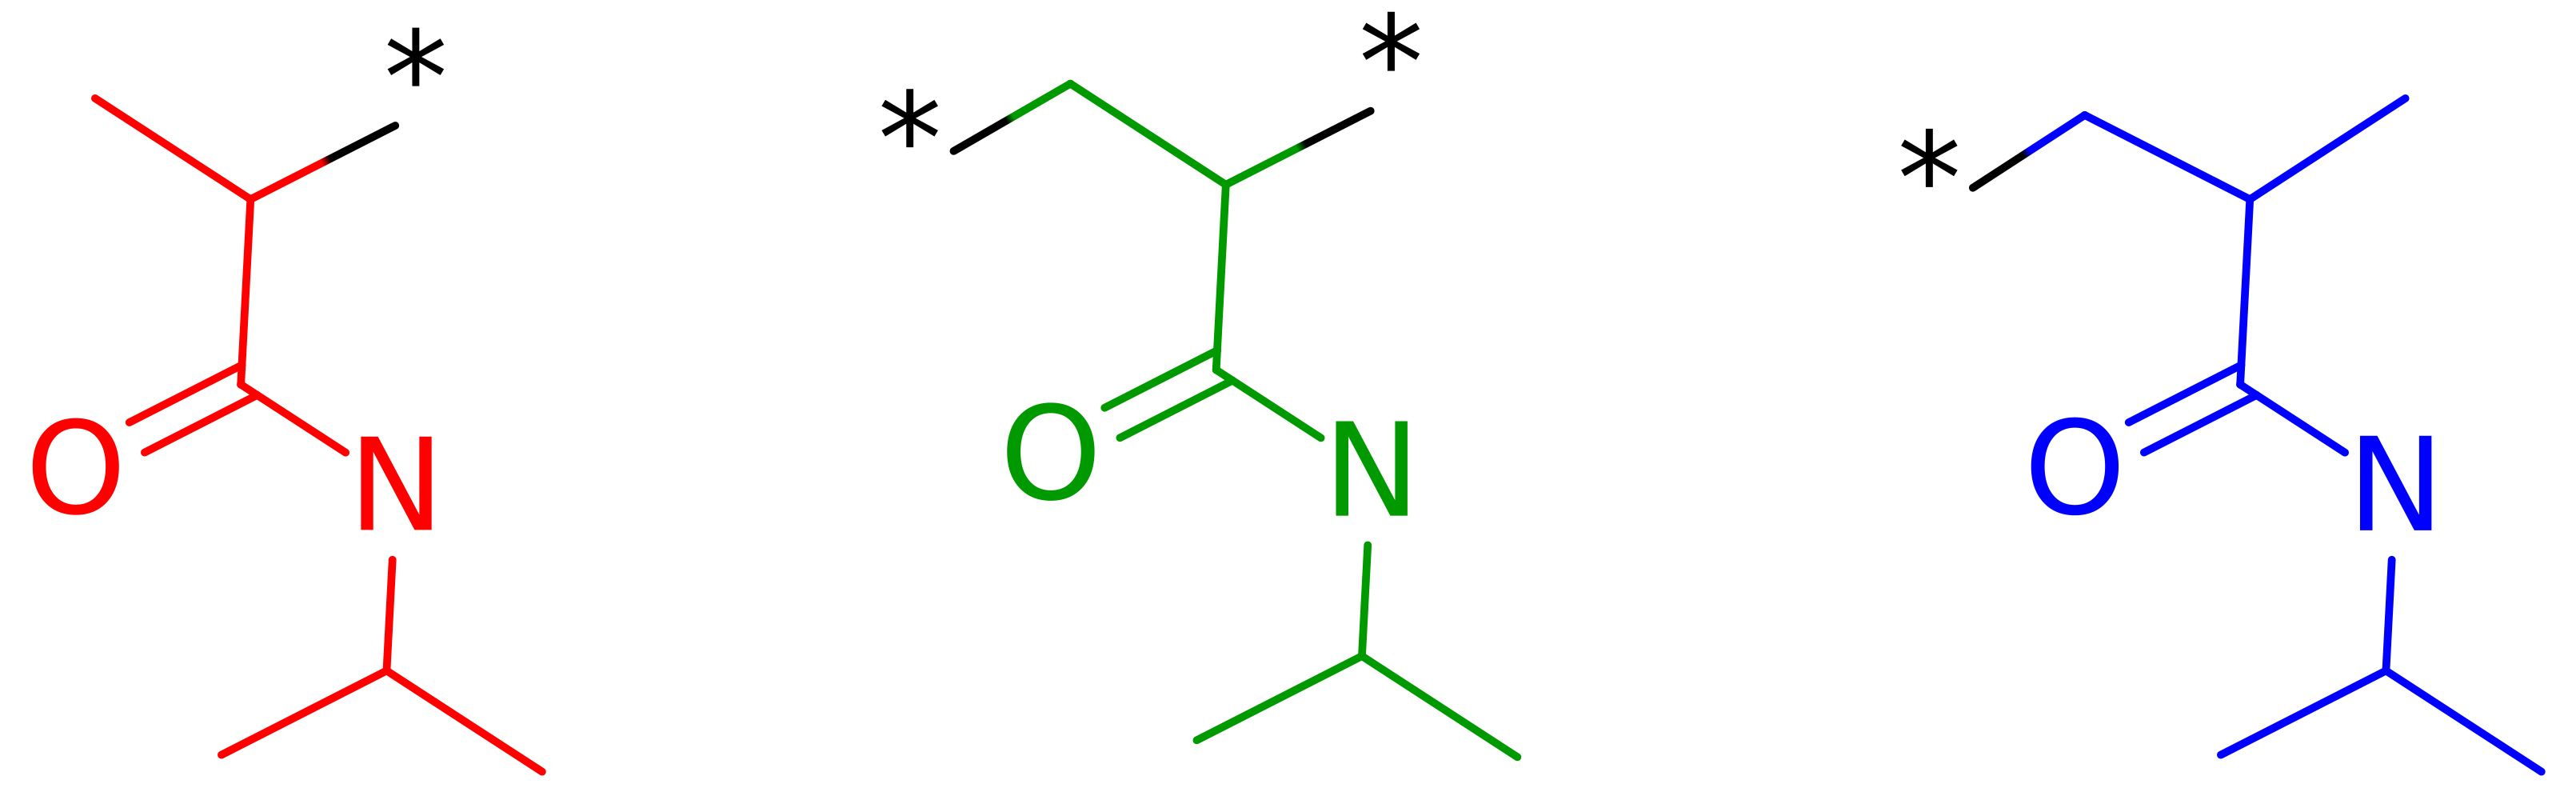
\includegraphics[width=\textwidth]{PNIPAM/PNIPAMBBs.png}
    \caption{The BBs for building PNIPAM molecules that were used in this tutorial.}
    \label{fig:PNIPAMBBs}
\end{figure}


Where \texttt{bb\_PNIP-start.itp}, \texttt{bb\_PNIP.itp} and \texttt{bb\_PNIP-end.itp} are the first, the repeated monomer and the last BBs, respectively.
The \texttt{list\_param.itp} is the parameters file and it should be written according to the selected force field.
The \texttt{connect.in} file is the connectivity file.
In this file, one should define the used BBs and how they are connected.
Using a smaller polymer connectivity file as an example, the \texttt{connect-5.in} file is provided with the following content:

\begin{lstlisting}
# Connectivity file to generate a PNIPAM with 5 monomers

#[ BUILDING BLOCKS ]
#BBNUM      BBNAME
  1     	PNIPS
  2     	PNIP
  3     	PNIP
  4	        PNIP
  5         PNIPE

#[ CONNECTS ]
#BBI    BBJ   IAT    JAT
 1       2     2      1
 2       3     2      1
 3       4     2      1
 4       5     2      1
\end{lstlisting}

In the field \texttt{[ BUILDING BLOCKS ]} the user should define the names of the BBs that will be used.
Those names should agree with the \texttt{[ moleculetype ]} within each BB.
Once the BBs are defined, the field \texttt{[ CONNECTS ]} has the information about which BBs are connected (using its index numbers defined in the previous field) and which atom in each BB is used to form the connection.
For example, according to line the line 13: \texttt{1       2     2      1} the pyPolyBuilder will to create a covalent bond between the BBs 1 and 2 (the PNIPS and the first PNIP, respectively) using the atom 2 of the first BB, i.e., the PNIPS, and the atom 1 of the second BB, the first PNIP.
Consistently, this file contains the informations about what bonds to create in order to get the polymer built.

To build a PNIPAM with 5 monomer units, one can run the following code:

\begin{lstlisting}
python3 ../../../../__main__.py \
--bbs=bb_PNIP-start.itp,bb_PNIP.itp,bb_PNIP-end.itp \
--in=connect-5.in \
--params=list_param.itp \
--name=PNIPAM \
--output=PNIPAM.itp \
--gro=PNIPAM.gro \
--network
\end{lstlisting}

Note that the \texttt{--network} was explicitly invoked and that all the BBs are passed at once using the \texttt{--bbs} option to be used by the \texttt{connect.in} file.

Once the optimization step is gone, the PNIPAM MTF will be ready and an initial guess for the coordinates file will be provided.
It is important to note that this guess is evaluated in vaccum and a further energy minimization step is highly advisable to be carried out in a proper molecular dynamics package.

\begin{figure}
    \center
    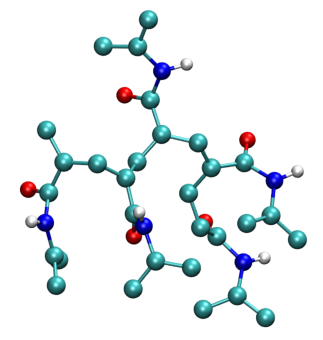
\includegraphics[width=0.5\textwidth]{PNIPAM/PNIPAMPPB.pdf}
    \caption{PNIPAM polymer with 5 monomers created by pyPolyBuilder.}
    \label{fig:PNIPAMPPB}
\end{figure}

Since pyPolyBuilder optmization steps are made in vacuum, the geometry (Figure \ref{fig:PNIPAMPPB}) may not be in the same conformation than in solution.
To carry a small simulation in water, the run directory is provided.
Copy the output from pyPolyBuilder \texttt{PNIPAM.*} to \texttt{run} and edit the \texttt{PNIPAM.sh} script to use the correct gromacs path on your machine.
By running \texttt{PNIPAM.sh}, the molecule generated by pyPolyBuilder (\texttt{PNIPAM.gro}) will be solvated in water, equilibrated and simulated for 100 ps.
After equilibrated, PNIPAM conformation can be seen in Figure \ref{fig:PNIPAMSOL}.

\begin{figure}
    \center
    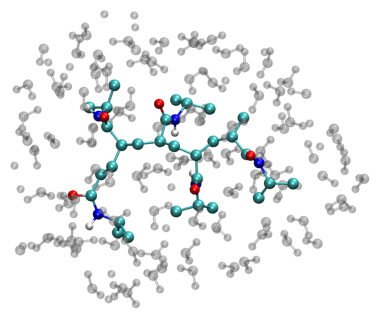
\includegraphics[width=0.5\textwidth]{PNIPAM/PNIPAMSOL.pdf}
    \caption{PNIPAM polymer with 5 monomers in water.}
    \label{fig:PNIPAMSOL}
\end{figure}

Changing the size of the polymer is not as easy as using dendrimer module.
However it is still easily doable.
Due to pyPolyBuilder philosophy, all connections are defined in a single file, hence, in order to make more connections, one only needs to edit the connectivity file.
Within this tutorial directory, two connectivity files were provided: \texttt{connect-5.in} and \texttt{connect.in}.
The former connects 5 monomers of the PNIPAM polymer, while the later uses the same three BBs to build a 30-mer.
Using the \texttt{connect.in} as the connectivity file, one can simply run the code:

\begin{lstlisting}
python3 ../../../../__main__.py \
--bbs=bb_PNIP-start.itp,bb_PNIP.itp,bb_PNIP-end.itp \
--in=connect.in \
--params=list_param.itp \
--name=PNIPAM \
--output=PNIPAM.itp \
--gro=PNIPAM.gro \
--network
\end{lstlisting}

That is very similar to the previous one.
In fact, only the \texttt{--in} option was changed.
Both built polymers can be seen in Figure \ref{fig:PNIPAMSIZE}.

\begin{figure}
    \center
    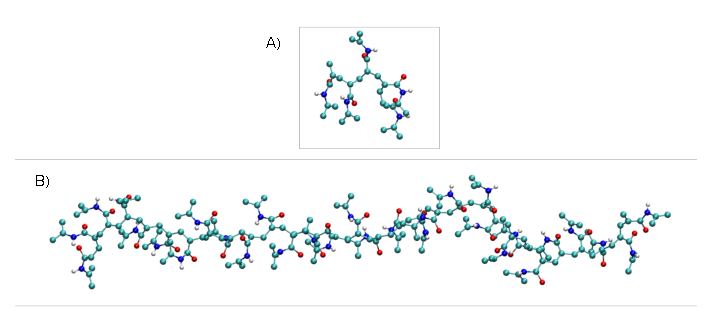
\includegraphics[width=\textwidth]{PNIPAM/PNIPAMSIZE.pdf}
    \caption{PNIPAM polymers created by pyPolyBuilder.
    These two polymers were used to illustrate the simplicity of using pyPolyBuilder for varying the size of the created molecule. A) is a PNIPAM with only 5 monomers while B) is a PNIPAM with 30 monomers.
    The same BBs were used for both polymers.}
    \label{fig:PNIPAMSIZE}
\end{figure}
\clearpage

% \subsubsection{poly_p-benzamide}
% \input{Poly_Benzamide/PBZ}

% \subsubsection{Cyclic polymer}
% \input{Cyclic_Pol/Cyclic_Pol}


\subsection{Advanced examples}
For some complex cases, it may be necessary to combine both modules to build different parts of the molecule separately. 
In the following tutorials parts of the molecule were built using the dendrimer module and the network module was used to connect them.
Generally, these tasks may also be realized with the network module alone since it is completely generic, however, the dendrimer module is specialized to build any dendritic structure and it is desirable to use it to ease the process.

\subsubsection{PAMAM/PPI-half}

Similarly to the PAMAM/PPI-Janus (see Section \ref{PAMAM/PPI-Janus}), this tutorial aims to build a dendrimer in which each side of the dendrimer is composed by BBs of a different dendrimer.
However, differently to the PAMAM/PPI-Janus tutorial, here the molecule is supposed to be completely divided between PAMAM and PPI side.
That is, even the core block is split (Figure \ref{fig:Half}).

\begin{figure}
    \centering
    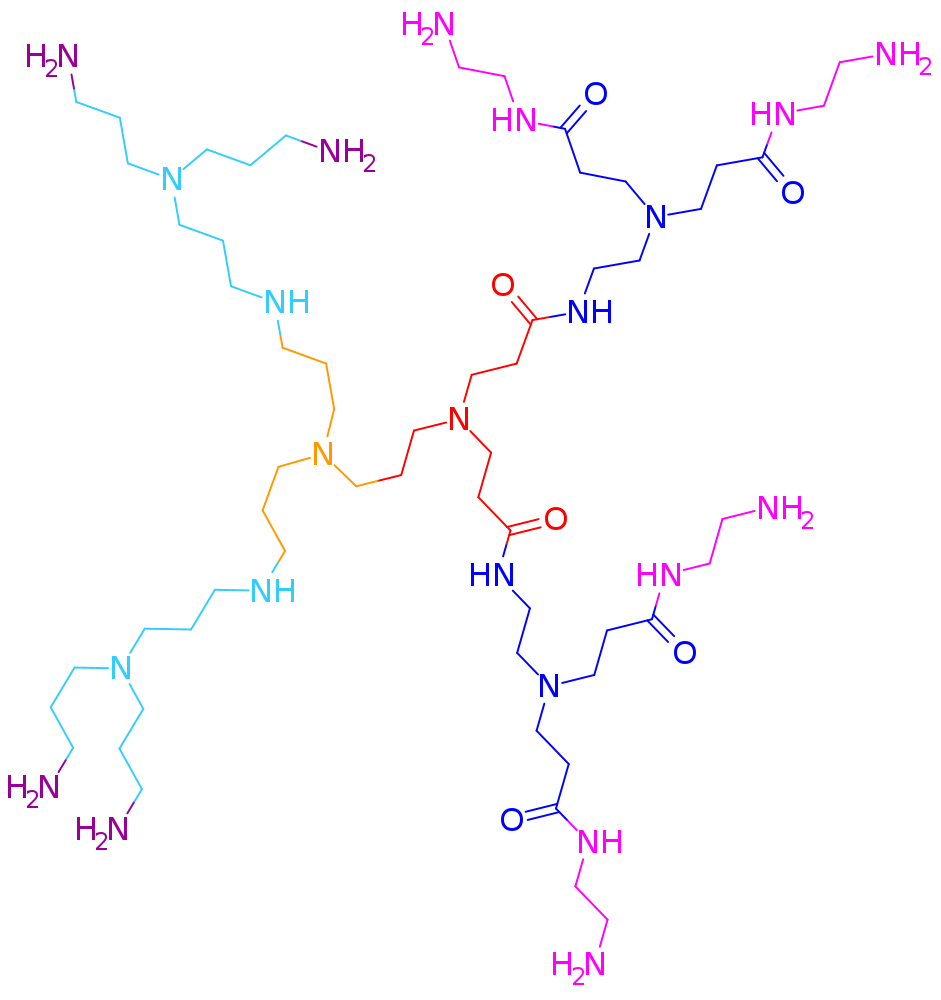
\includegraphics[width=0.4\textwidth]{PAMAM_PPI-half/PAMAMPPIPOL.png}
    \caption{PAMAM/PPI dendrimer in which each side is composed by either PAMAM or PPI dendrimer. The PAMAM core block is illustrated in red, intermediary and core blocks are displayed in blue and pink, respectively. PPI part is displayed in orange, cyan and purple for core, intermediary and terminal BBs, respectively. }
    \label{fig:Half}
\end{figure}

All needed files are provided in demo directory:

\begin{lstlisting}
<path/to/pypolybuilder>/demo/gromacs_format/polymer/PAMAM_PPI_Half
\end{lstlisting}
\dirtree{%
.1 PAMAM\_PPI\_Half.
.2 coreHalf\_PAMAM.itp.
.2 coreHalf\_PPI.itp.
.2 inter\_PAMAM.itp.
.2 inter\_PPI.itp.
.2 ter\_PAMAM.itp.
.2 ter\_PPI.itp.
.2 list\_param.itp.
.2 connect.in.
.2 run.
.3 PAMAM\_PPI\_Half.sh.
.3 PAMAMPPI.top.
.3 mdp.
}

All the following procedure for building the molecule with a side using only PAMAM BBs and the other side using only PPI BBs, is automated in a available bash file called \texttt{how\_to\_run\_this\_example.txt}.

In order to do that, we created separated topology files of the core block for each side of the dendrimer, \texttt{coreHalf\_PAMAM.itp} and \texttt{coreHalf\_PPI.itp}.
Intermediary and terminal blocks are the same as used in PAMAM and PPI tutorials (See Figure \ref{fig:HalfBBs}).

\begin{figure}
    \centering
    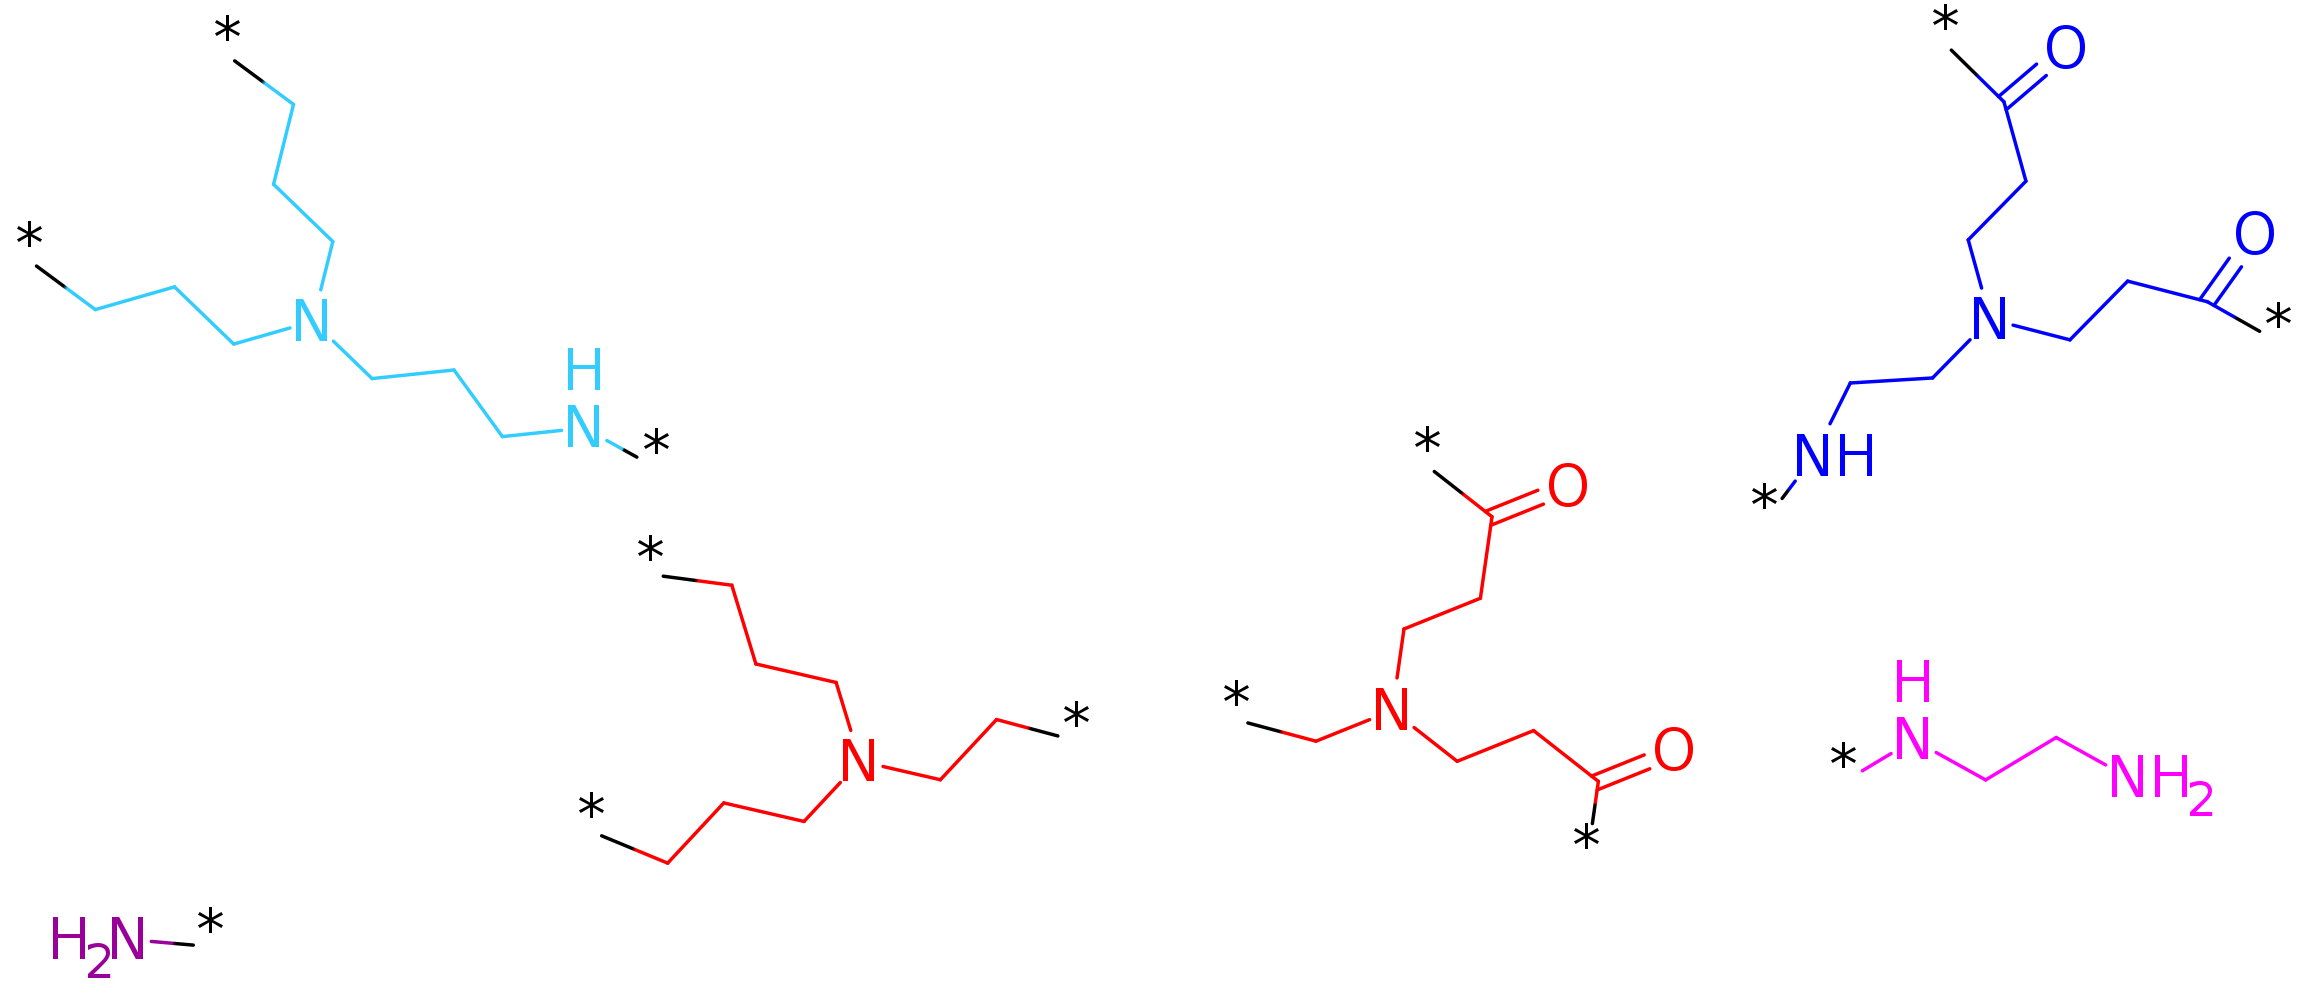
\includegraphics[width=\textwidth]{PAMAM_PPI-half/PAMAMPPIBBs.png}
    \caption{PAMAM/PPI dendrimer in which each side is composed of PAMAM or PPI. PAMAM BBs are illustrated on the right where the core block is illustrated in red, intermediary and core blocks are displayed in blue and pink, respectively. PPI part is on the left and displayed in orange, cyan and purple for core, intermediary and terminal BBs, respectively.}
    \label{fig:HalfBBs}
\end{figure}

Therefore, firstly each half will be built using the dendrimer module by using the following command lines:

\begin{lstlisting}
python3 ../../../../__main__.py \
--core=coreHalf_PAMAM.itp \
--inter=inter_PAMAM.itp \
--ter=ter_PAMAM.itp \
--params=list_param.itp \
--ngen=1 \
--name=PAMH \
--output=PAMAMhalf.itp \
--nogeom \
--dendrimer
\end{lstlisting}

To build the first side using PAMAM BBs.
Here the usage of dendrimer module is exactly the same as when generating a whole dendrimer.
The only difference is that at the core BB, the \texttt{[ branches ]} field tells pyPolyBuilder that only the two available branching points will be used.

\begin{lstlisting}
[ branches ]
;  donor   acceptor
    0      6
    0      9
\end{lstlisting}

Secondly, PPI half is built.
The procedure is similar to the one for building the PAMAM half:

\begin{lstlisting}
python3 ../../../../__main__.py \
--core=coreHalf_PPI.itp \
--inter=inter_PPI.itp \
--ter=ter_PPI.itp \
--params=list_param.itp \
--ngen=1 \
--name=PPIH \
--output=PPIhalf.itp \
--nogeom
\end{lstlisting}

In both calls of pyPolyBuilder, the option \texttt{--nogeom} was used since we're not interested in optimizing the geometry for an intermediary molecule. 
Hence, this options can be used to save time skipping the optimization step and the generation of a coordination file for the intermediary molecules.

\begin{figure}
    \centering
    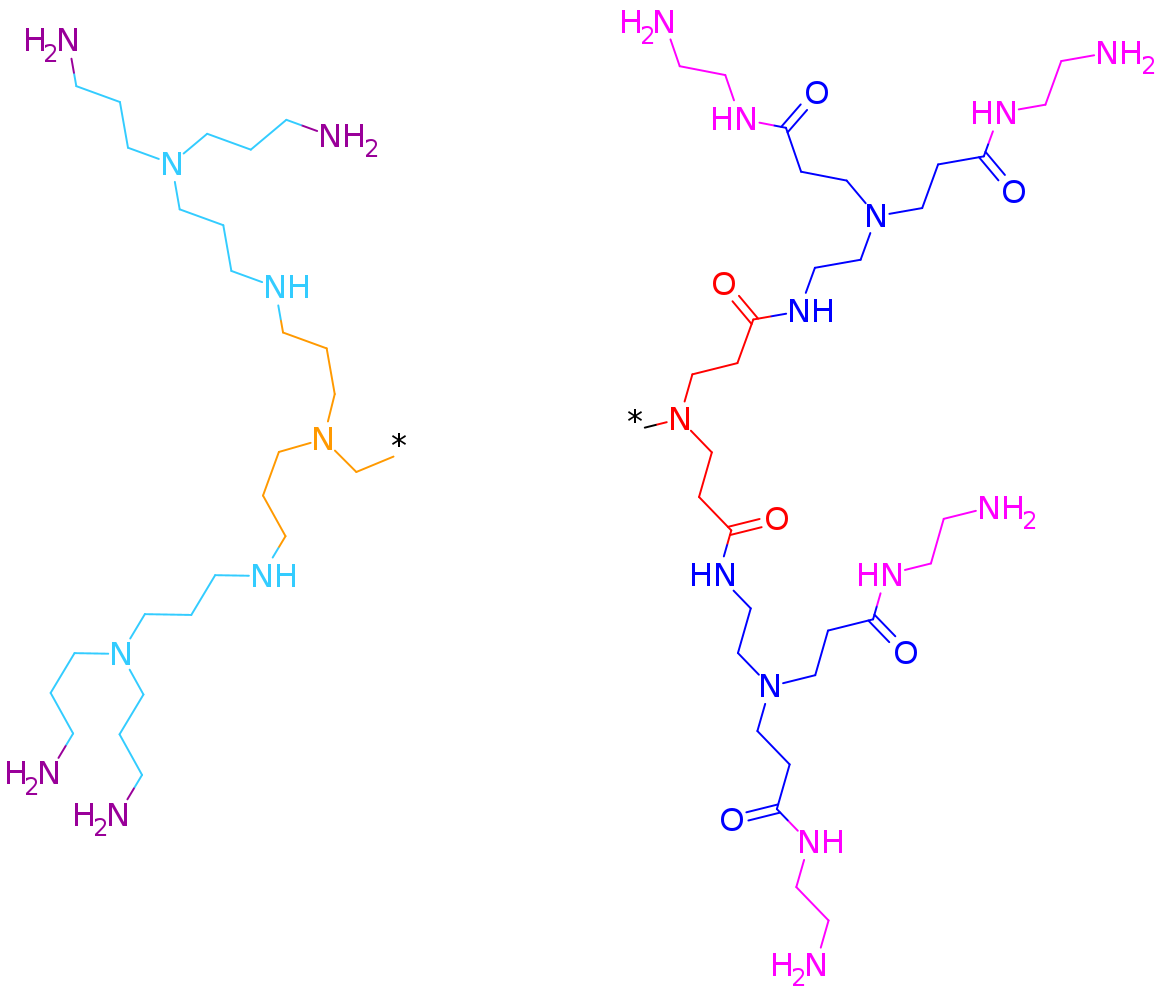
\includegraphics[width=0.5\textwidth]{PAMAM_PPI-half/PAMAMPPIHalfs.png}
    \caption{PAMAM/PPI dendrimer in which each side is composed by either PAMAM or PPI dendrimer. The PAMAM core block is illustrated in red, intermediary and core blocks are displayed in blue and pink, respectively. PPI part is displayed in orange, cyan and purple for core, intermediary and terminal BBs, respectively. }
    \label{fig:HalfHalf}
\end{figure}

Once both halfs are done, one will have the MTFs for each side of the dendrimer (see Figure \ref{fig:HalfHalf}.
Now these two parts need to be connected by using the network module.
In order to do that, the \texttt{connect.in} file simply uses both sides and connect the fist atom of each topology.

\begin{lstlisting}
#[ BUILDING BLOCKS ]
1       PAMH
2       PPIH

#[ CONNECTS ]
1       2       1       1
\end{lstlisting}

Connecting both sides, the final molecule will be generated (Figure \ref{fig:HalfHalf}).
The command line to connect the dendrimer is the following one:

\begin{lstlisting}
python3 ../../../../__main__.py \
--bbs=PAMAMhalf.itp,PPIhalf.itp \
--in=connect.in \
--params=list_param.itp \
--name=PAMPPI \
--output=PAMAMPPI.itp \
--gro=PAMAMPPI.gro \
--nsteps 500 \
--network
\end{lstlisting}

Once this last command line is executed, the dendrimer will be readily prepared, including its geometry optimized in vacuum (Figure \ref{fig:HalfPPB}).
In this tutorial, the internal pseudo-force field of pyPolyBuilder was used, so it is strongly suggested that after building any molecule in pyPolyBuilder, a MD simulation package should be used to minimize the energy using an actual force field (if the option \texttt{--forcefield} was not used in pyPolyBuilder) and to equilibrate the molecule in the desired solvent.

\begin{figure}
    \centering
    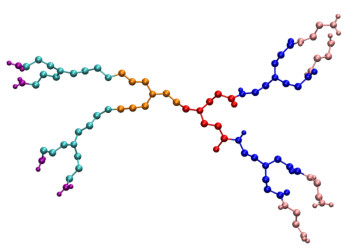
\includegraphics[width=0.5\textwidth]{PAMAM_PPI-half/PAMAMPPIPPB.pdf}
    \caption{PAMAM/PPI dendrimer in which each side is composed by either PAMAM or PPI dendrimer. The PAMAM core block is illustrated in red, intermediary and core blocks are displayed in blue and pink, respectively. PPI part is displayed in orange, cyan and purple for core, intermediary and terminal BBs, respectively. }
    \label{fig:HalfPPB}
\end{figure}

To mimic the procedure of energy minimization, equilibration and simulation, the run directory was provided where the script \texttt{PAMAM\_PPI\_half.sh} can be used to automate the whole process.
The outputs from pyPolyBuilder \texttt{PAMAMPPI.*} need to be copied to the run directory and the \texttt{PAMAM\_PPI\_half.sh} need to be changed to include an actual path for a gromacs package.
By running \texttt{PAMAM\_PPI\_half.sh}, it will automatically solvate the molecule, minimize the energy of the system, equilibrate it for 100 ps in nvt and npt ensembles and carry out 100 ps of molecular dynamics simulation.
An equilibrated structure is shown in Figure \ref{fig:HalfSOL}.

\begin{figure}
    \centering
    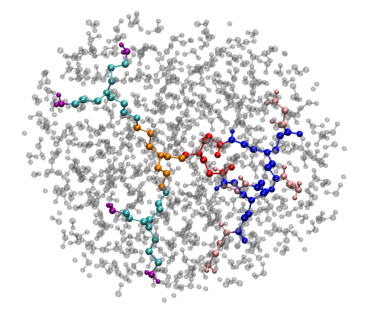
\includegraphics[width=0.5\textwidth]{PAMAM_PPI-half/PAMAMPPISOL.pdf}
    \caption{PAMAM/PPI dendrimer in which each side is composed of either PAMAM or PPI in water. The color scheme for the dendrimer is in accordance with Figure \ref{fig:HalfPPB} and water molecules are translucent in silver.}
    \label{fig:HalfSOL}
\end{figure}
\clearpage

\subsubsection{PEG connected PAMAM dendrimer}

This tutorial aims to generate a molecule in which two halfs of a PAMAM dendrimer are connected by a Poly-ethylenegycol (PEG) linker.
Similarly to the PAMAM/PPI-Half tutorial, this tutorial needs to use both modules in order to prepare the molecule conveniently (Figure \ref{fig:PAMAMPEG}).

\begin{figure}
    \centering
    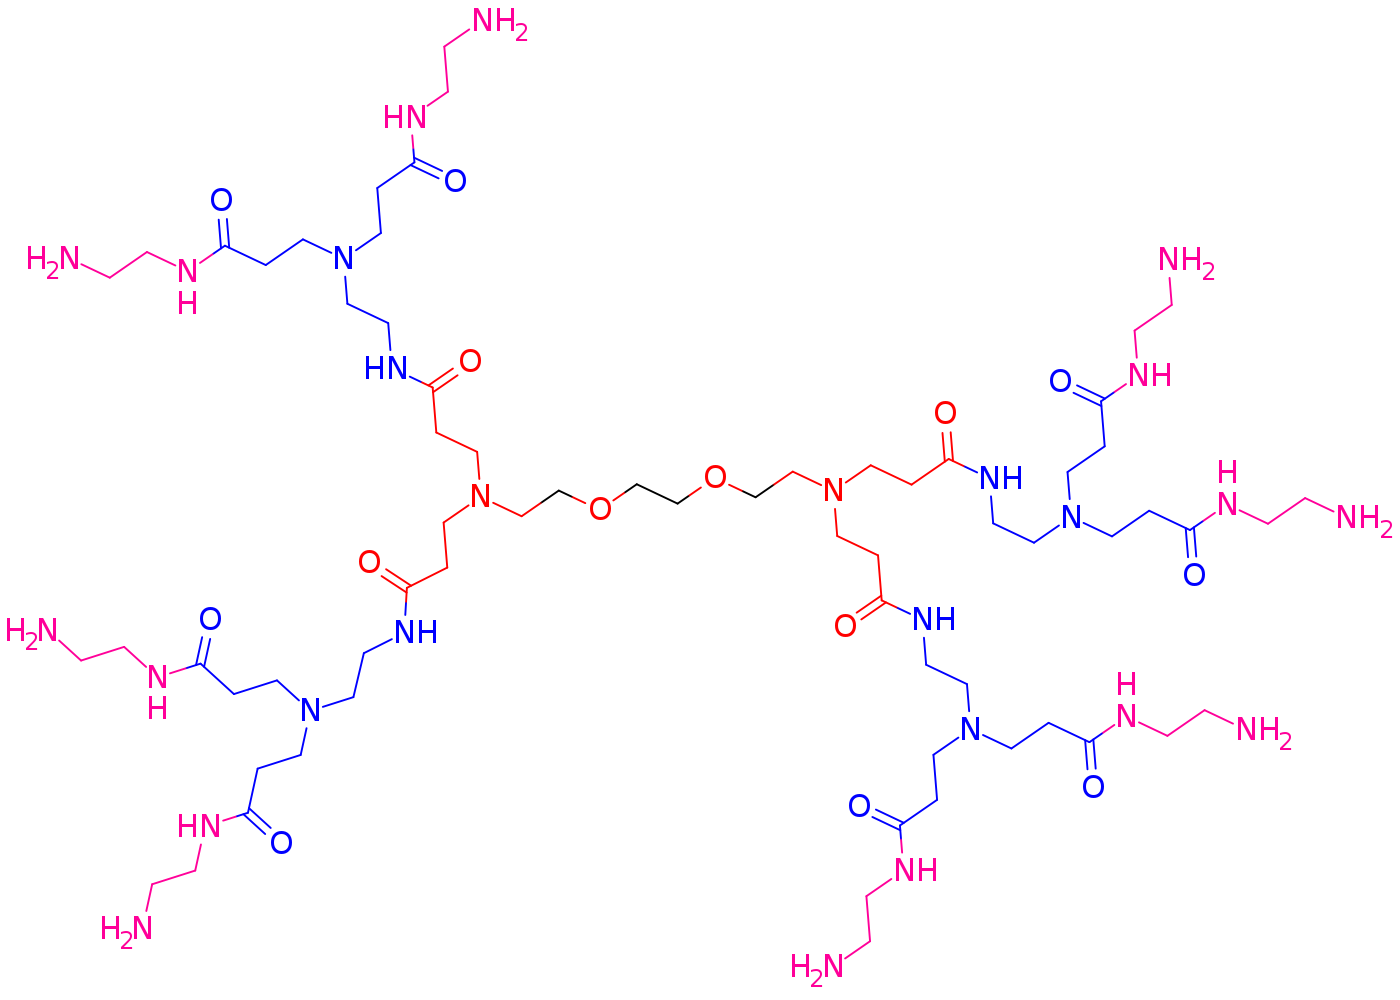
\includegraphics[width=0.5\textwidth]{PAMAM_PEG/PAMAMPEG.png}
    \caption{PAMAM-PEG dendrimer in which each side is connected by a PEG polymer. The PAMAM core block is illustrated in red, intermediary and core blocks are displayed in blue and pink, respectively. The PEG moiety of the molecule is placed between the two PAMAM halfs.}
    \label{fig:PAMAMPEG}
\end{figure}

All needed files are provided in demo directory:

\begin{lstlisting}
<path/to/pypolybuilder>/demo/gromacs_format/polymer/PAMAM_PolyEtyleneglycol
\end{lstlisting}
\dirtree{%
.1 PAMAM\_PolyEtyleneglycol.
.2 coreHalf\_PAMAM.itp.
.2 inter\_PAMAM.itp.
.2 ter\_PAMAM.itp.
.2 ethyleneglycol.itp.
.2 list\_param.itp.
.2 connect.in.
.2 run.
.3 PAMAM\_PEG.sh.
.3 PAMAM\_PEG.top.
.3 mdp.
}

All the following procedure for building the PAMAM dendrimer, in which its core is split into two halfs connected by a PEG polymer, is automated in the available bash script \texttt{how\_to\_run\_this\_example.txt}.

For building this molecule, we will make the dendritic part of the molecule first and then connect two of these, using the network module to get all BBs together.
The core BB for the dendrimer module is a PAMAM core split in the middle.
Intermediary and terminal blocks are the same as used in PAMAM tutorial (See Figure \ref{fig:PAMAMPEGBBs}).

\begin{figure}
    \centering
    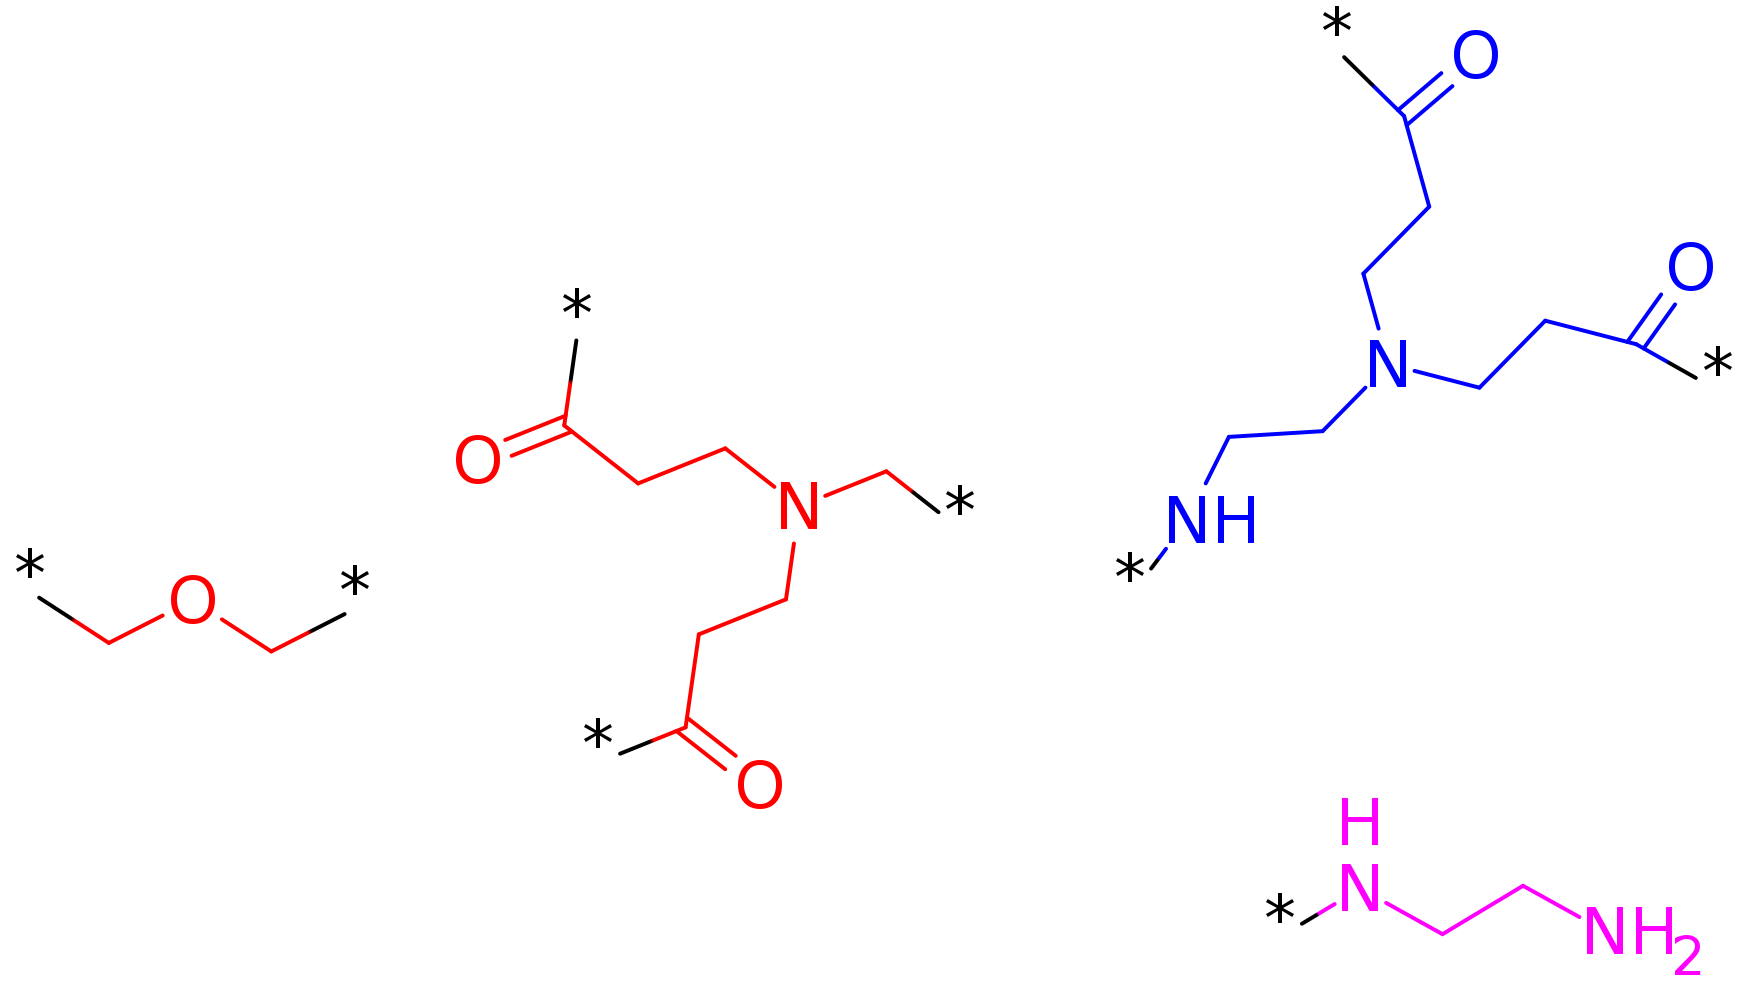
\includegraphics[width=0.6\textwidth]{PAMAM_PEG/PAMAMPEGBBs.png}
    \caption{PAMAM-PEG dendrimer BBs. The PAMAM core, intermediary and terminal blocks are displayed in red, blue and pink, respectively. The PEG monomer is placed on the left of the figure.}
    \label{fig:PAMAMPEGBBs}
\end{figure}

The dendrimer module can be called to generate the dentritic part of the molecule by using the following command line to build the first part of the molecule using PAMAM BBs:

\begin{lstlisting}
python3 ../../../../__main__.py \
--core=coreHalf_PAMAM.itp \
--inter=inter_PAMAM.itp \
--ter=ter_PAMAM.itp \
--params=list_param.itp \
--ngen=1 \
--name=PAMH \
--output=PAMAMhalf.itp \
--nogeom \
--dendrimer
\end{lstlisting}

Here the usage of dendrimer module is exactly the same as when generating a whole dendrimer.
However, the \texttt{[ branches ]} field is made in a way that pyPolyBuilder uses only the two available branching points.

\begin{lstlisting}
[ branches ]
;  donor   acceptor
    0      6
    0      9
\end{lstlisting}

In the first pyPolyBuilder call, the option \texttt{--nogeom} was used because we are not interested in optimizing the geometry of a molecule, which is only an intermediate step of building the final MTF.
Hence, this options can be used to save time skipping the optimization stage and the generation of a coordinates file for the intermediary molecules.

\begin{figure}
    \centering
    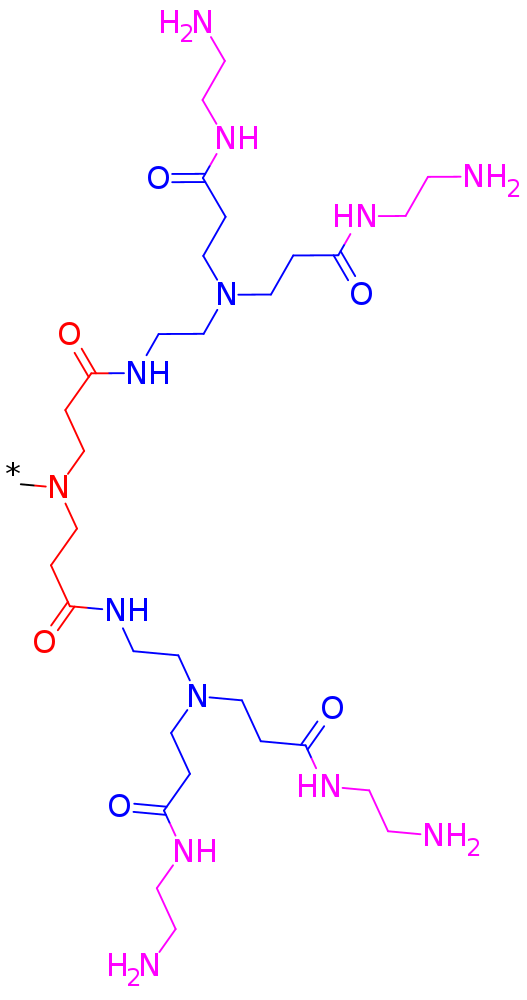
\includegraphics[width=0.3\textwidth]{PAMAM_PEG/PAMAMPEGHalf.png}
    \caption{PAMAM part of the PAMAM-PEG dendrimer. The color scheme is adopted in accordance with the Figure \ref{fig:PAMAMPEGBBs}.}
    \label{fig:PAMAMPEGHalf}
\end{figure}

Once we have built the dendritic part of the molecule (Figure \ref{fig:PAMAMPEGHalf}), the network module can be called to connect every BB we need.
For instance, we will use the blocks in Figure \ref{fig:PAMAMPEGBBs} to build the molecule in Figure \ref{fig:PAMAMPEG}.
In order to do that, the \texttt{connect.in} file defines how the BBs are connected.
To make it simple, only two monomers of PEG will be used.

\begin{lstlisting}
#[ BUILDING BLOCKS ]
1   PAMH
2   EG
3   EG
4   PAMH

#[ CONNECTS ]
1    2    1    1
2    3    3    1
3    4    3    1

\end{lstlisting}

After building all the BBs, the final molecule will be done and can be visualized in any software (Figure \ref{fig:PAMAMPEGHalf}).
The command line to gather all BBs together is the following one:

\begin{lstlisting}
python3 ../../../../__main__.py \
--bbs=PAMAMhalf.itp,etyleneglycol.itp \
--in=connect.in --params=list_param.itp \
--name=PAMPEG --output=PAMAM_PEG.itp \
--gro=PAMAM_PEG.gro \
--network
\end{lstlisting}

Once this last command line is done, the dendrimer will be completed, including its geometry optimized in vacuum (Figure \ref{fig:PAMAMPEGPPB}).
It is strongly suggested that the geometry generated by pyPolyBuilder be energy-minimized in a simulation package.
The procedure of energy minimization, equilibration, and simulation, is automated in a script file called \texttt{PAMAM\_PEG.sh} in the run directory.

\begin{figure}
    \centering
    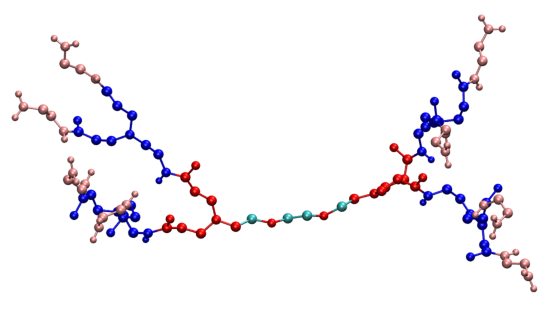
\includegraphics[width=0.5\textwidth]{PAMAM_PEG/PAMAM_PEG_PPB.pdf}
    \caption{PAMAM\_PEG dendrimer in which each side is connected by a PEG linker. The PAMAM core block is illustrated in red, intermediary and core blocks are displayed in blue and pink, respectively. The PEG moiety of the molecule is placed between the two PAMAM halfs.}
    \label{fig:PAMAMPEGPPB}
\end{figure}

The outputs from pyPolyBuilder \texttt{PAMAM\_PEG.*} needs to be copied to the run directory and the input path for the gromacs package in the \texttt{PAMAM\_PEG.sh} needs to be changed.
\texttt{PAMAM\_PEG.sh} can be run in order to automatically solvate the molecule, minimize the energy of the system, equilibrate it for 100 ps in nvt and npt ensembles, and carry out 100 ps of molecular dynamics simulation.
Figure \ref{fig:PAMAMPEGSOL} shows a snapshot of an equilibrated conformation of the PAMAM-PEG molecule.

\begin{figure}
    \centering
    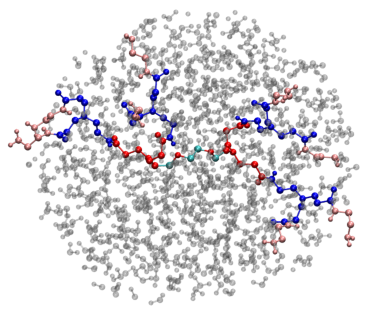
\includegraphics[width=0.5\textwidth]{PAMAM_PEG/PAMAM_PEG_SOL.pdf}
    \caption{PAMAM\_PEG dendrimer in water. The color scheme is in accordance with Figure \ref{fig:PAMAMPEGPPB}. The water molecules are displayed as translucent silver molecules.}.
    \label{fig:PAMAMPEGSOL}
\end{figure}
\clearpage

% \section*{Appendix}


\end{document}
